\section{系统测试}

\subsection{注册登录功能测试}

进入到智慧工厂管理系统之后,在上方导航栏处有登陆按钮,点击之后即可输入账号名与密码进行登录,对于初次使用本系统的工厂管理人员,在登录界面有方有注册按钮,即可对当前部门组织进行注册。注册时填入注册所需提供的信息之后点击注册按钮,若注册信息填写有误,例如用户名已经被使用,则在上方发出错误信息提示,如图\ref{fig:rgster}所示。

\begin{figure}[H]
    \centering
    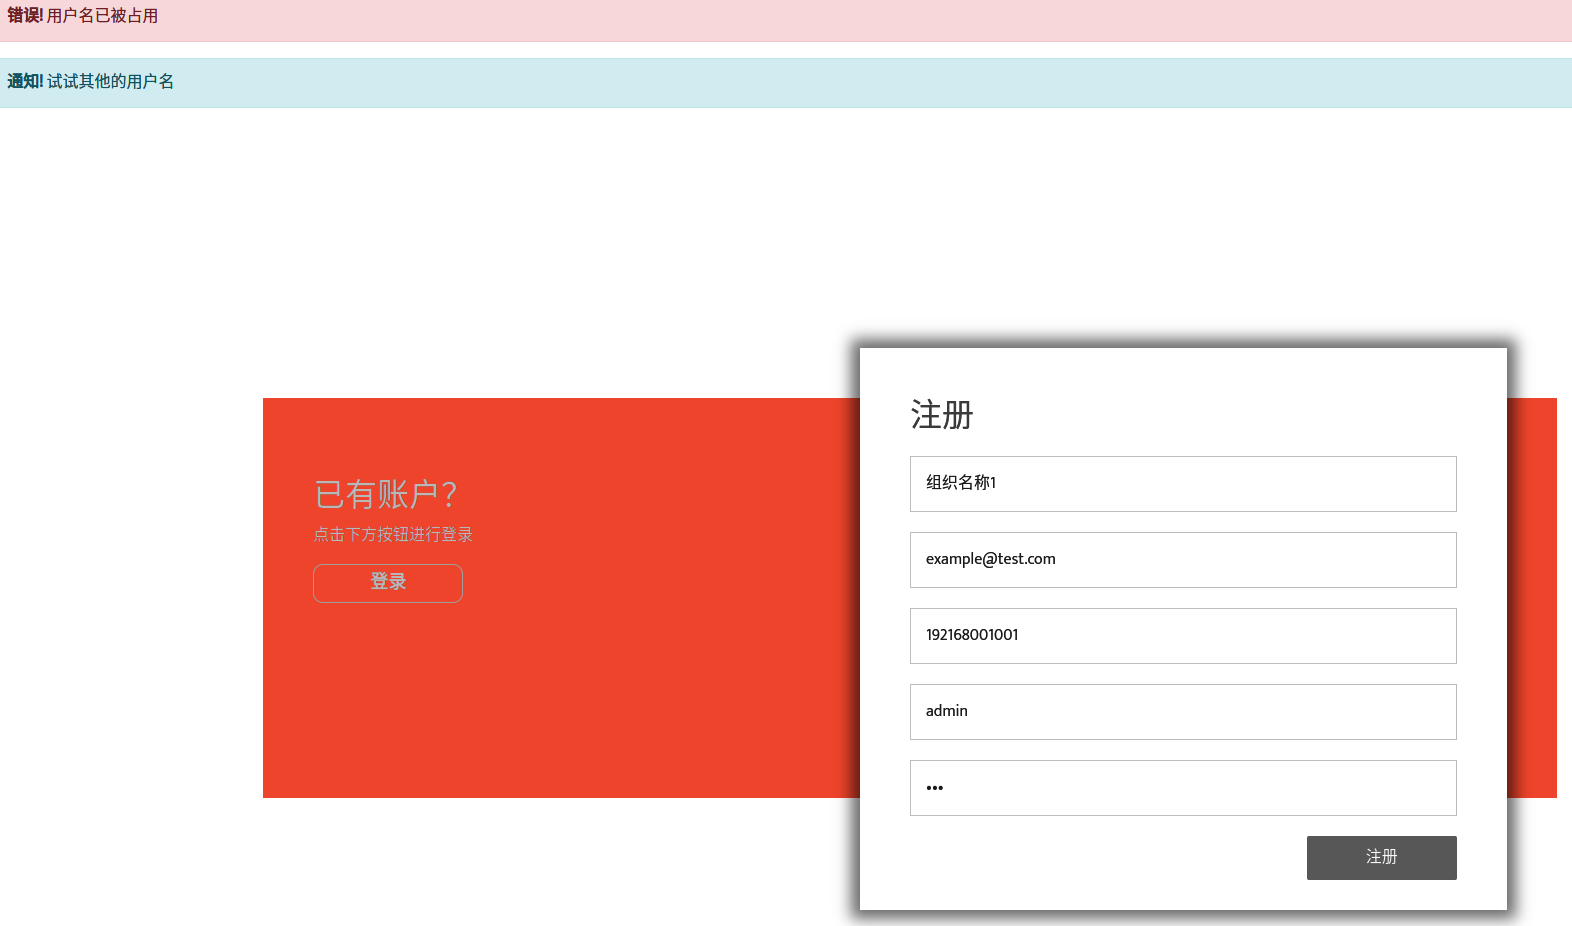
\includegraphics[width=.75\textwidth]{figures/6registererror.png}
    \caption{注册信息填入错误提示图}
    \label{fig:rgster}
\end{figure}

注册成功之后,在登录界面输入账户名与密码进行登录,登录成功之后,进入后台管理页面并且在上方显示欢迎用户的消息提示,如图\ref{fig:lgsccs}所示。

\begin{figure}[H]
    \centering
    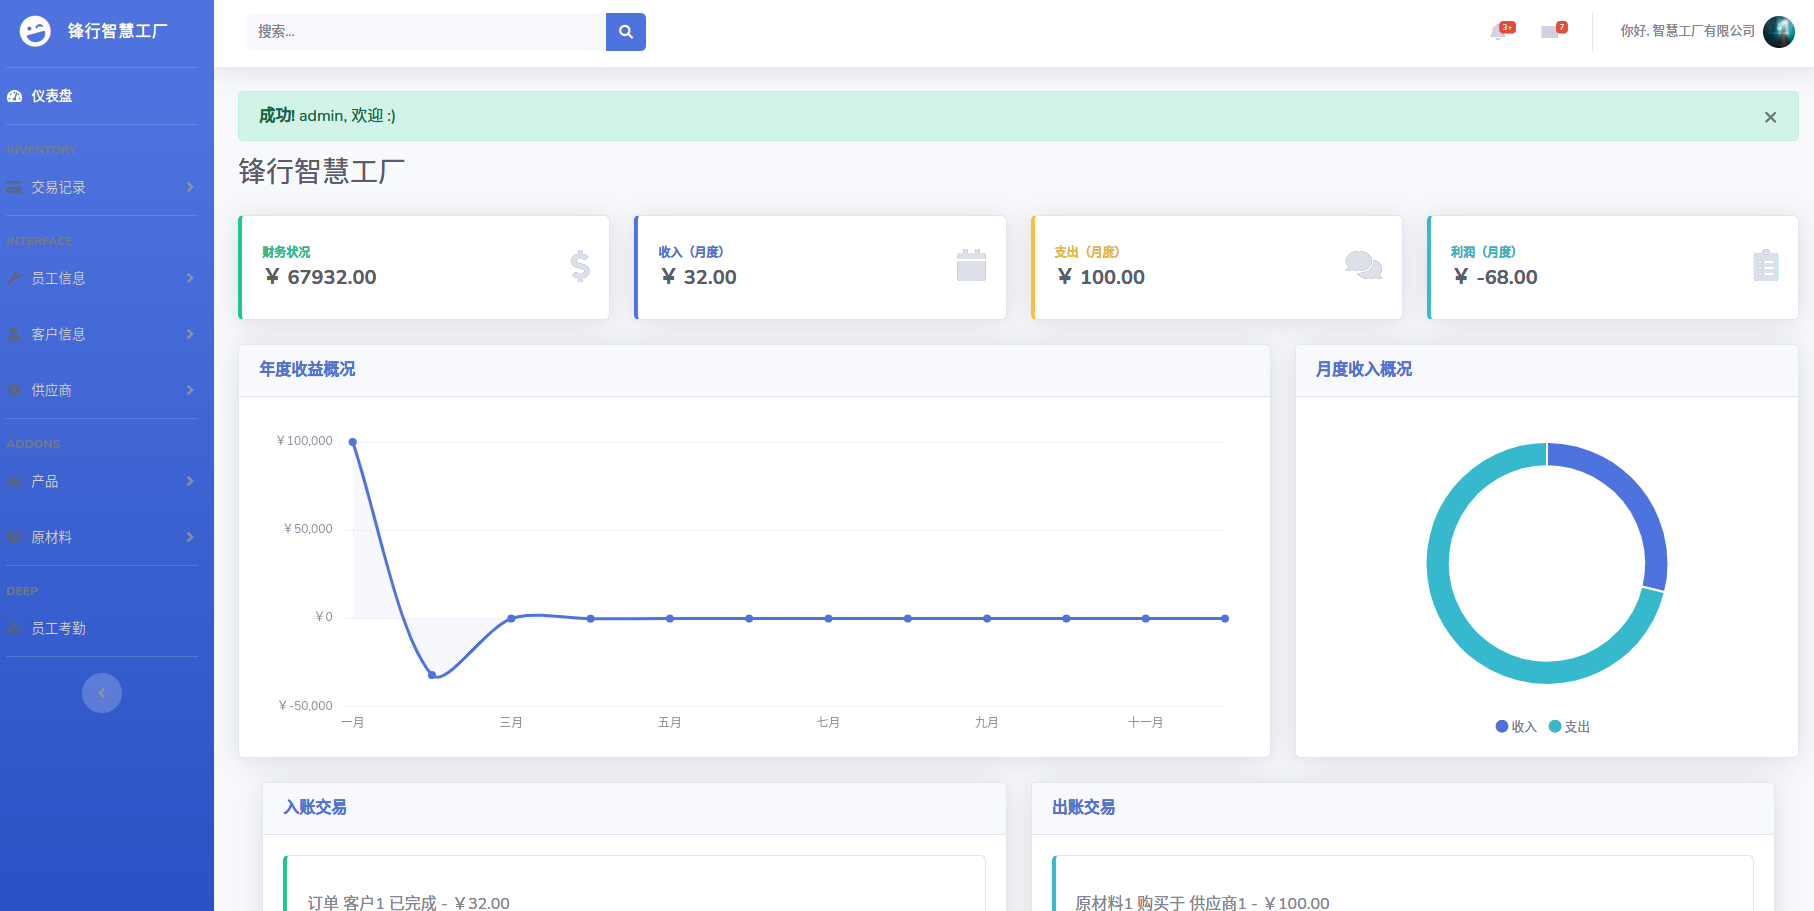
\includegraphics[width=.75\textwidth]{figures/6loginsuscess.png}
    \caption{登录成功消息提示图}
    \label{fig:lgsccs}
\end{figure}

\subsection{工厂信息管理测试}

进入后台管理页面之后,可以对当前工厂部门组织的信息进行管理,其中包括交易记录管理、员工信息管理、客户信息管理、供应商信息管理、产品信息管理以及原材料信息管理等。如图\ref{fig:tscttf}所示为交易记录的信息管理图。图\ref{fig:vuatsc}为查看所有交易记录详情,图\ref{fig:adnutsc}为添加交易记录页面。

\begin{figure}[H]
    \centering
    \begin{subfigure}{.45\textwidth}
        \centering
        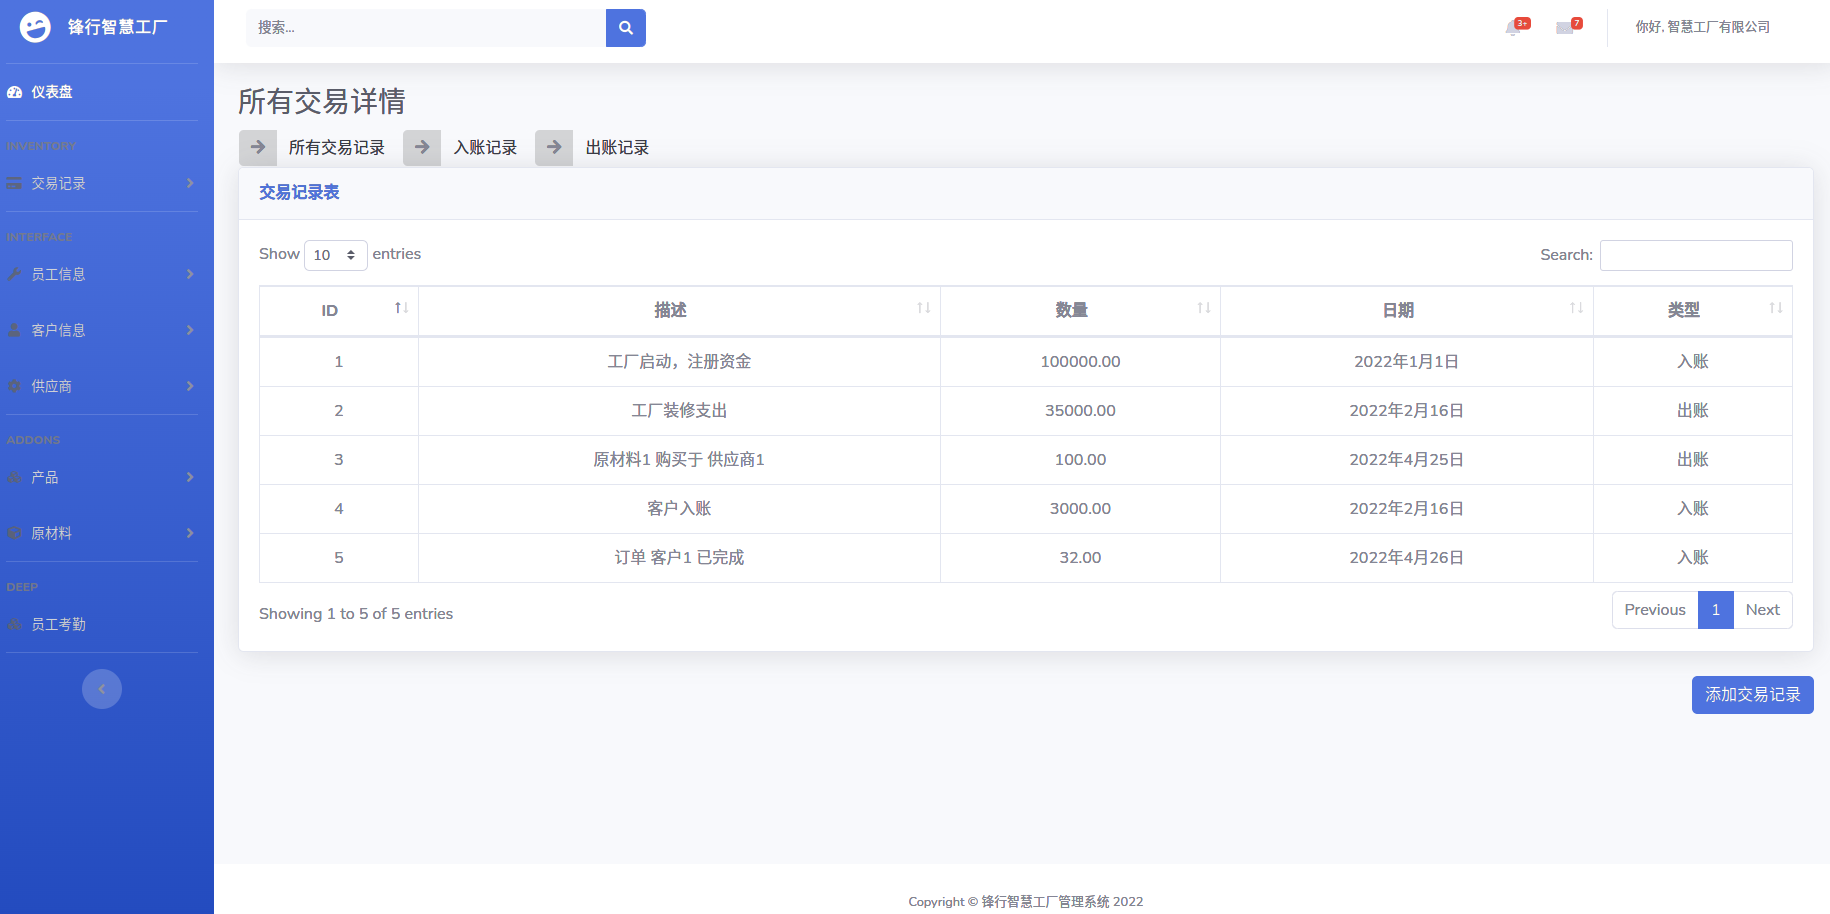
\includegraphics[width=\textwidth]{figures/6viewalltransc.png}
        \subcaption{查看交易记录详情图}
        \label{fig:vuatsc}
    \end{subfigure}
    \qquad
    \begin{subfigure}{.45\textwidth}
        \centering
        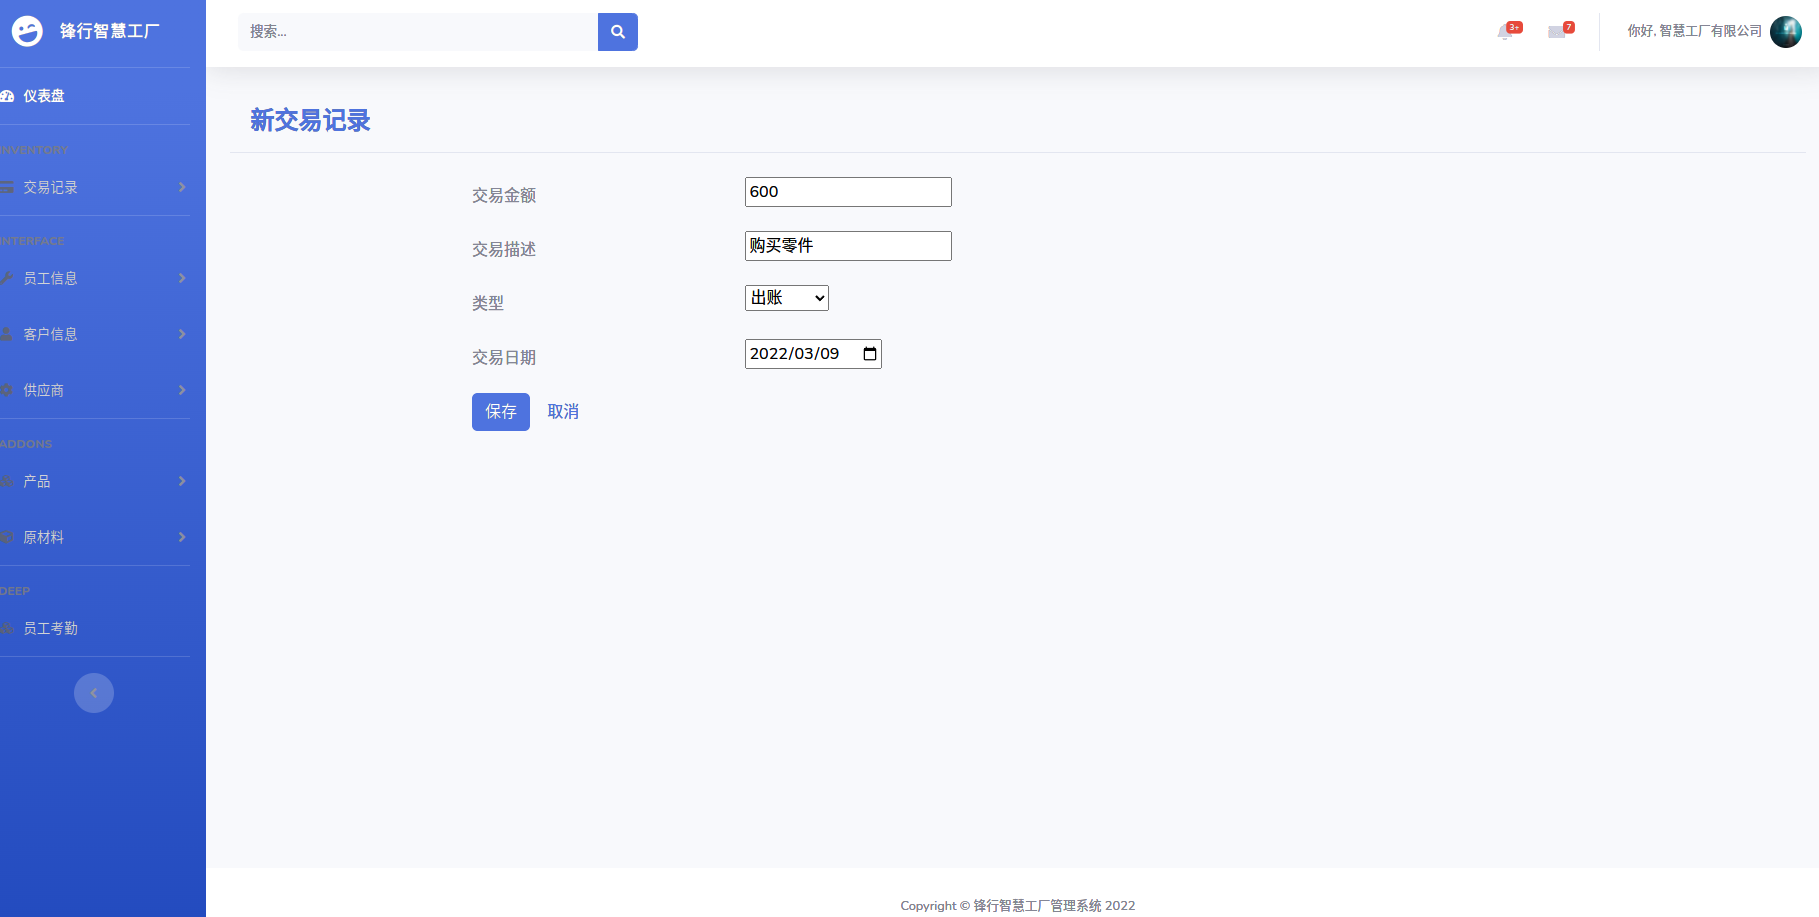
\includegraphics[width=\textwidth]{figures/6addnewtransc.png}
        \subcaption{添加交易记录测试图}
        \label{fig:adnutsc}
    \end{subfigure}
    \caption{交易记录信息管理测试图}
    \label{fig:tscttf}
\end{figure}

关于员工信息管理,包括查看员工、添加员工、支付薪资以及下单工作任务等功能,如图\ref{fig:emploetest}所示。图\ref{fig:vuaemple}为查看所有员工信息详情,图\ref{fig:adnuemploe}为添加员工页面功能测试,图\ref{fig:pyslr}为为员工支付当前月薪功能测试,图\ref{fig:addwork}为为指定员工指派工作任务功能测试。

\begin{figure}[H]
    \centering
    \begin{subfigure}{.45\textwidth}
        \centering
        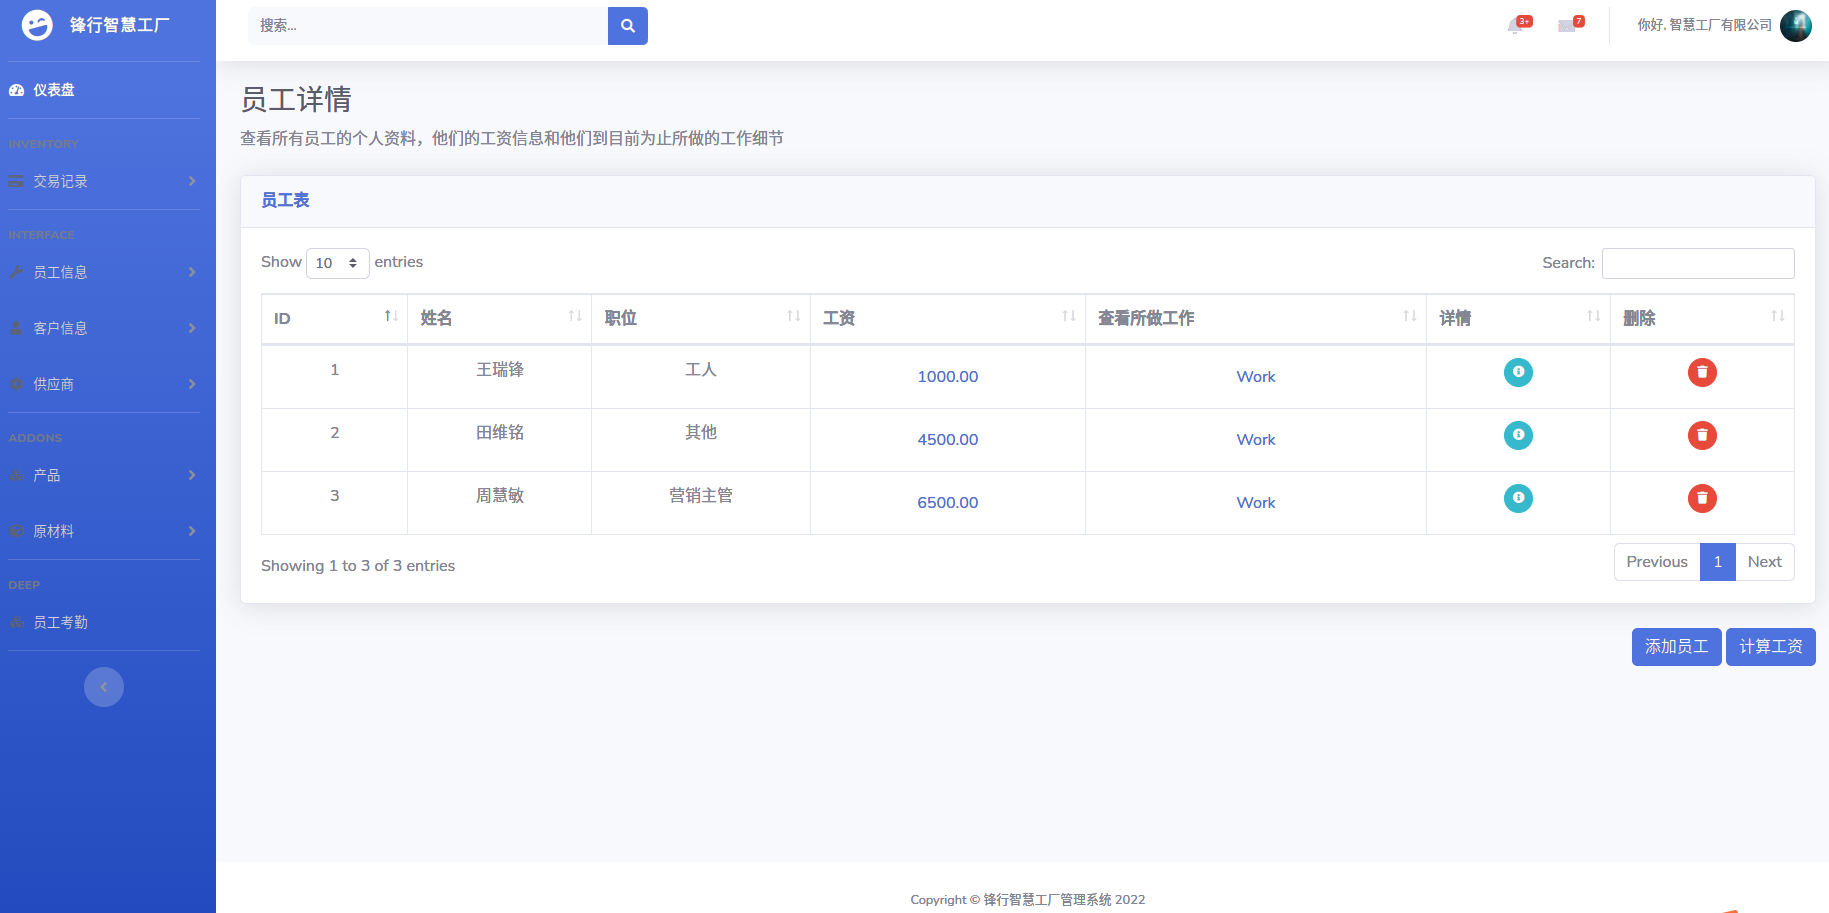
\includegraphics[width=\textwidth]{figures/6viewallemployee.png}
        \subcaption{查看员工信息详情图}
        \label{fig:vuaemple}
    \end{subfigure}
    \qquad
    \begin{subfigure}{.45\textwidth}
        \centering
        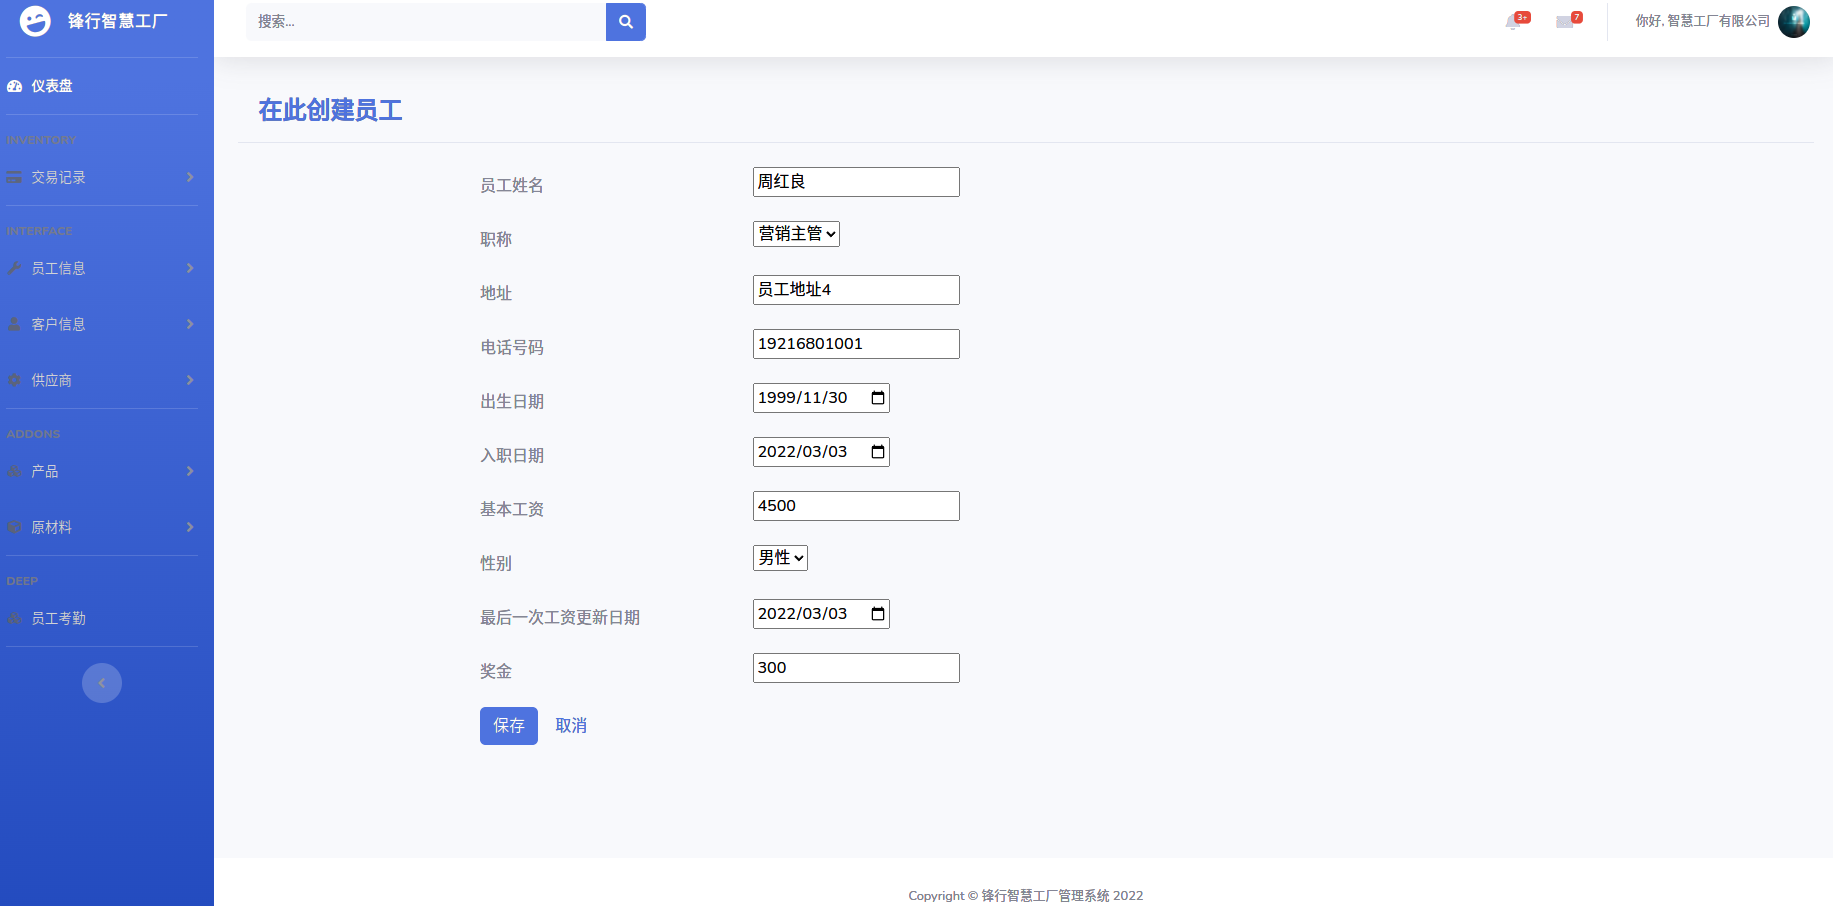
\includegraphics[width=\textwidth]{figures/6addnewemployee.png}
        \subcaption{添加员工测试图}
        \label{fig:adnuemploe}
    \end{subfigure}
    \\
    \begin{subfigure}{.45\textwidth}
        \centering
        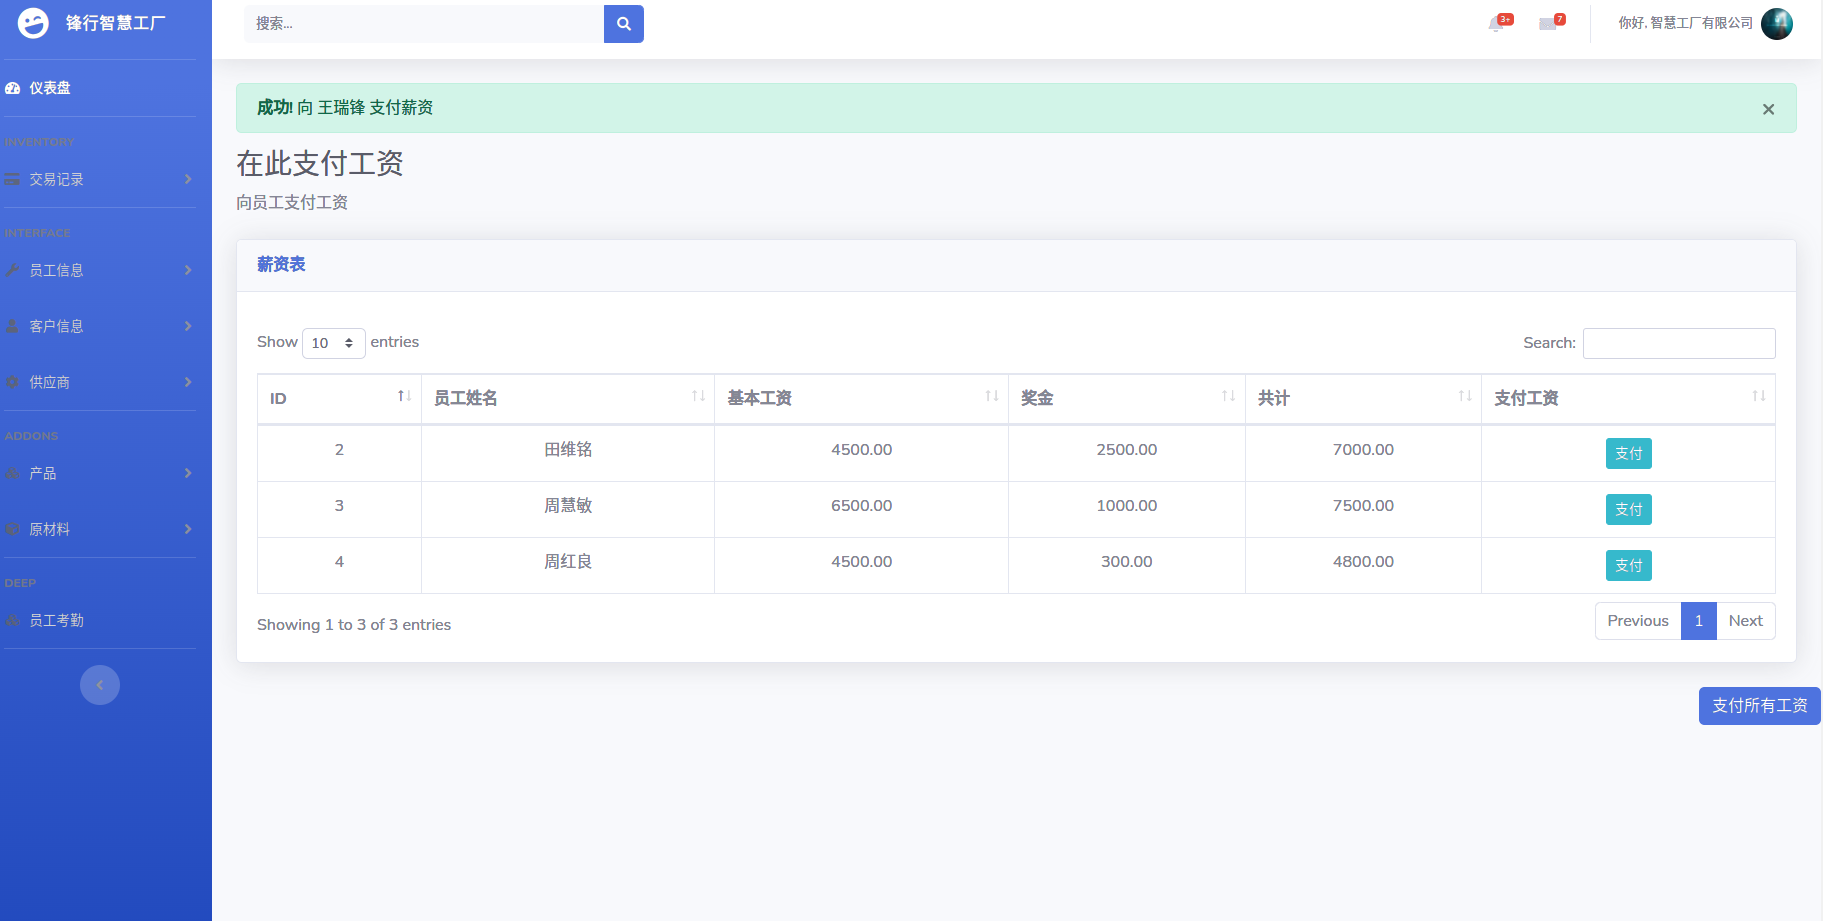
\includegraphics[width=\textwidth]{figures/6paysalary.png}
        \subcaption{向员工支付薪资测试图}
        \label{fig:pyslr}
    \end{subfigure}
    \qquad
    \begin{subfigure}{.45\textwidth}
        \centering
        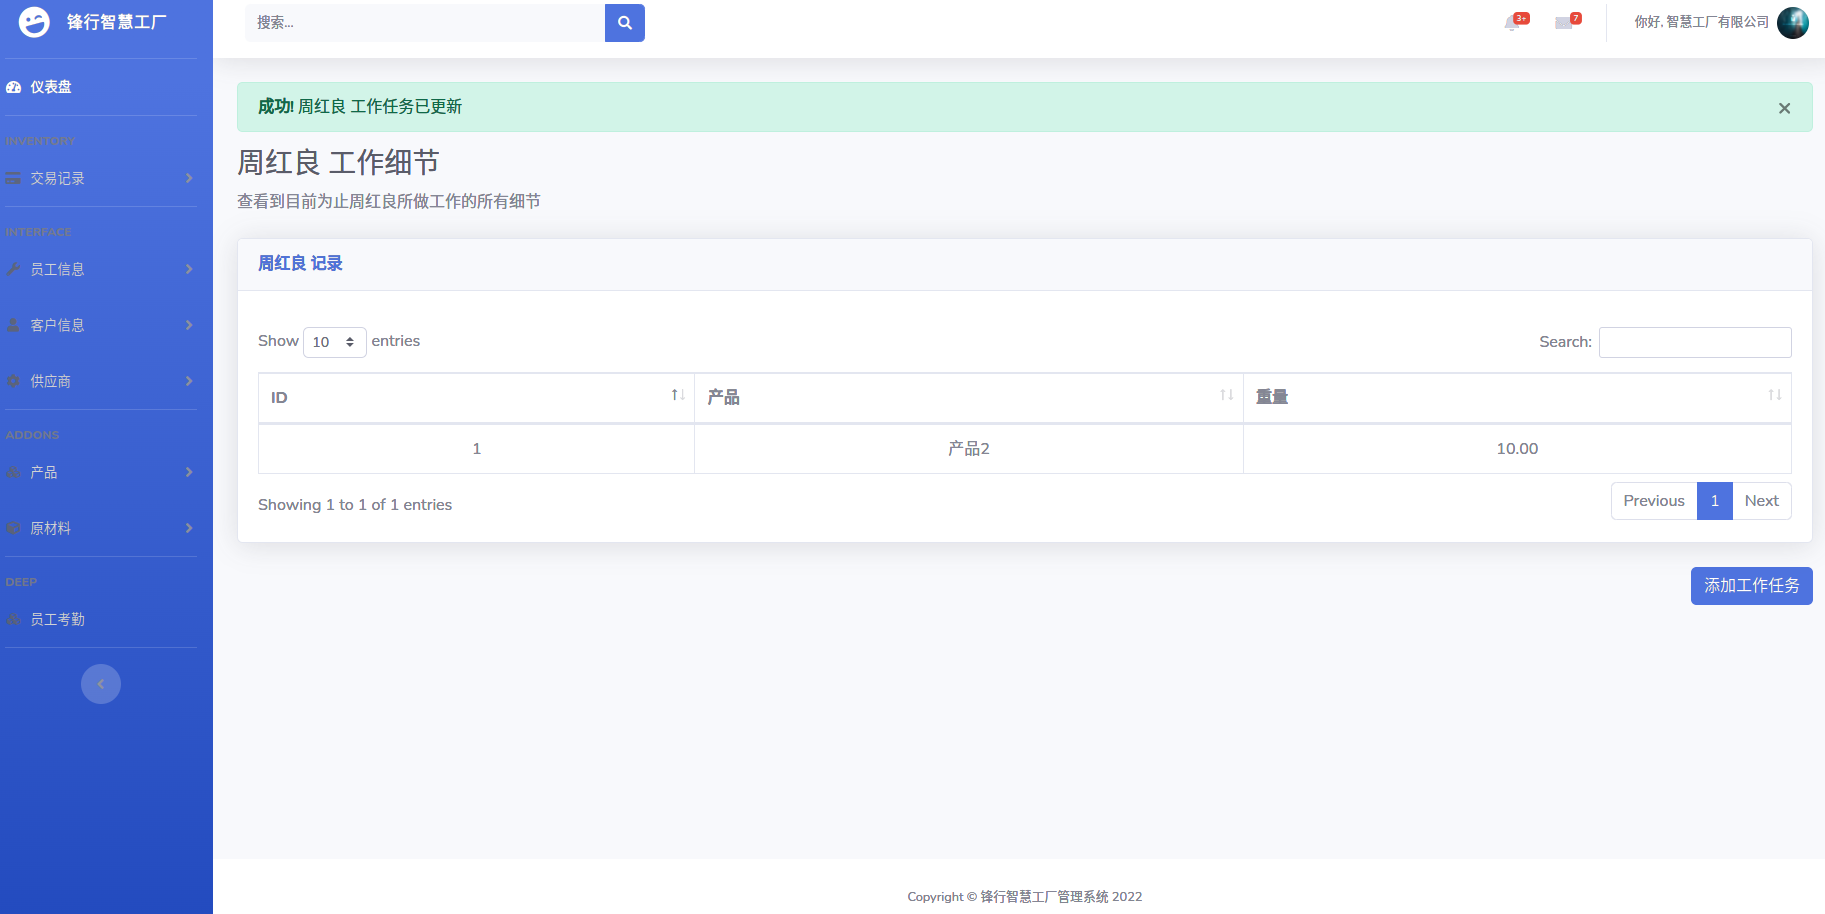
\includegraphics[width=\textwidth]{figures/6addwork.png}
        \subcaption{添加员工工作任务测试图}
        \label{fig:addwork}
    \end{subfigure}
    \caption{员工信息管理测试图}
    \label{fig:emploetest}
\end{figure}

客户信息管理包括查看所有客户信息详情、添加客户信息、为指定客户下单、查看客户信息订单以及订单详细收据等功能,如图\ref{fig:cstmtst}所示。图\ref{fig:vuacstm}为查看所有客户信息详情功能测试图,图\ref{fig:adnucstm}为添加客户信息功能测试,图\ref{fig:vuaods}为查看所有客户订单的功能测试,图\ref{fig:vuoddtls}为查看指定订单收据功能测试。

\begin{figure}[H]
    \centering
    \begin{subfigure}{.35\textwidth}
        \centering
        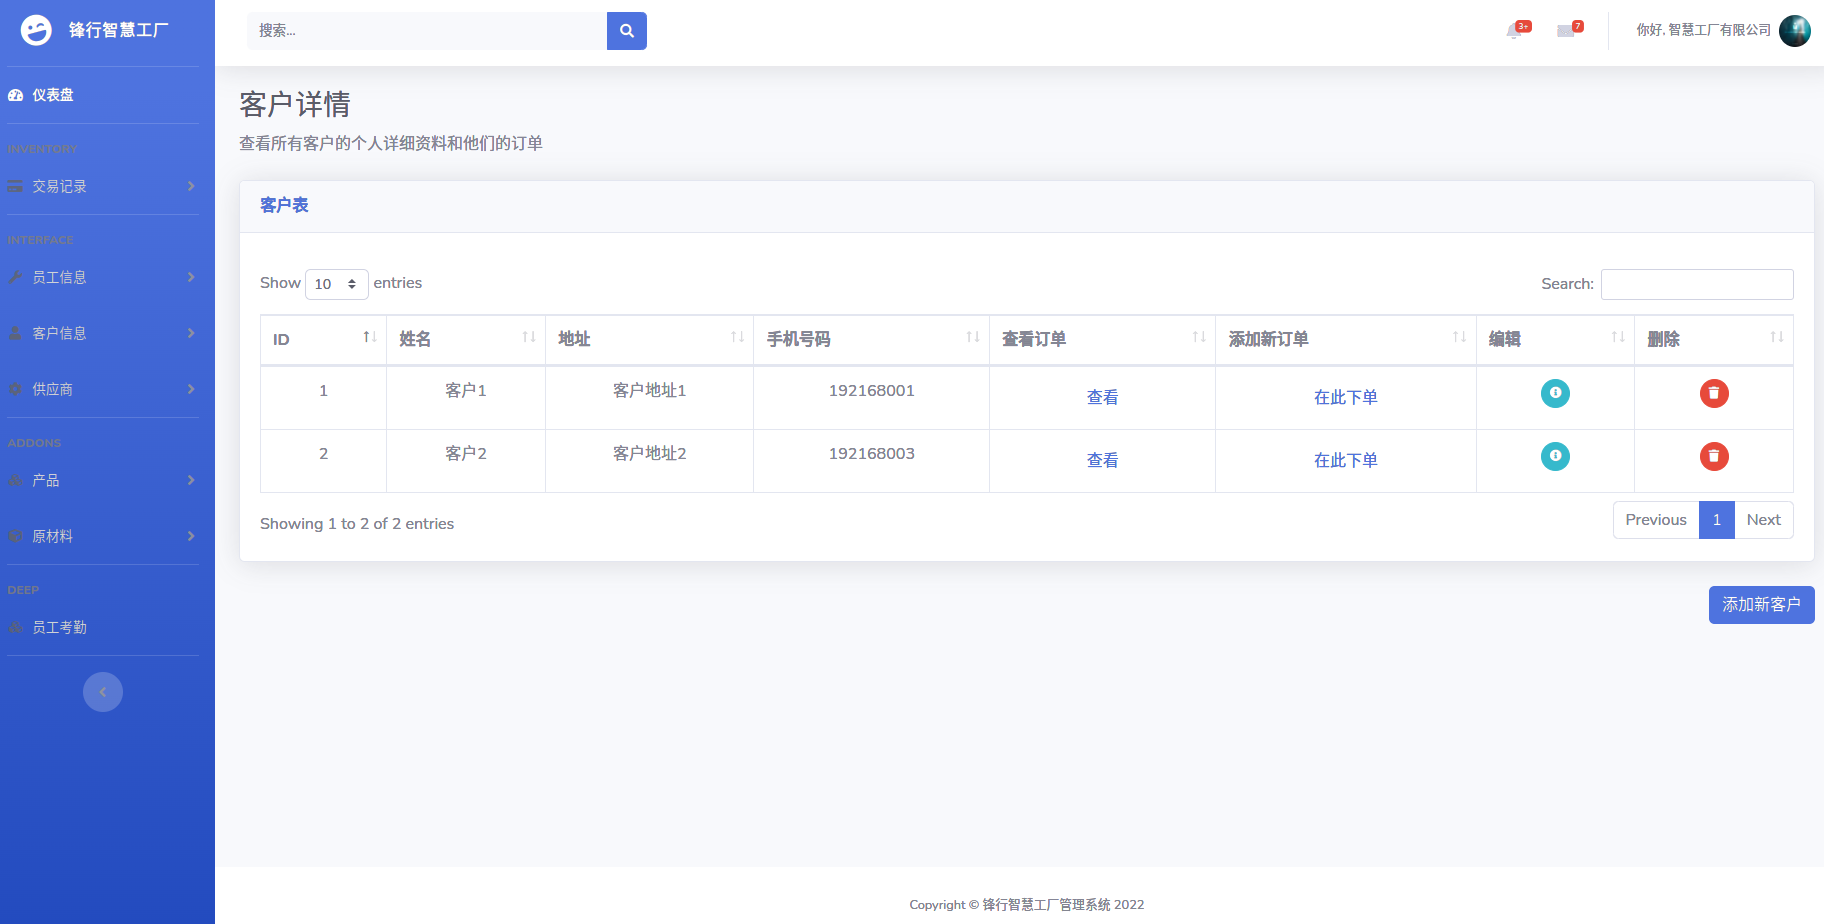
\includegraphics[width=\textwidth]{figures/6viewallcustomer.png}
        \subcaption{查看客户信息详情图}
        \label{fig:vuacstm}
    \end{subfigure}
    \qquad
    \begin{subfigure}{.35\textwidth}
        \centering
        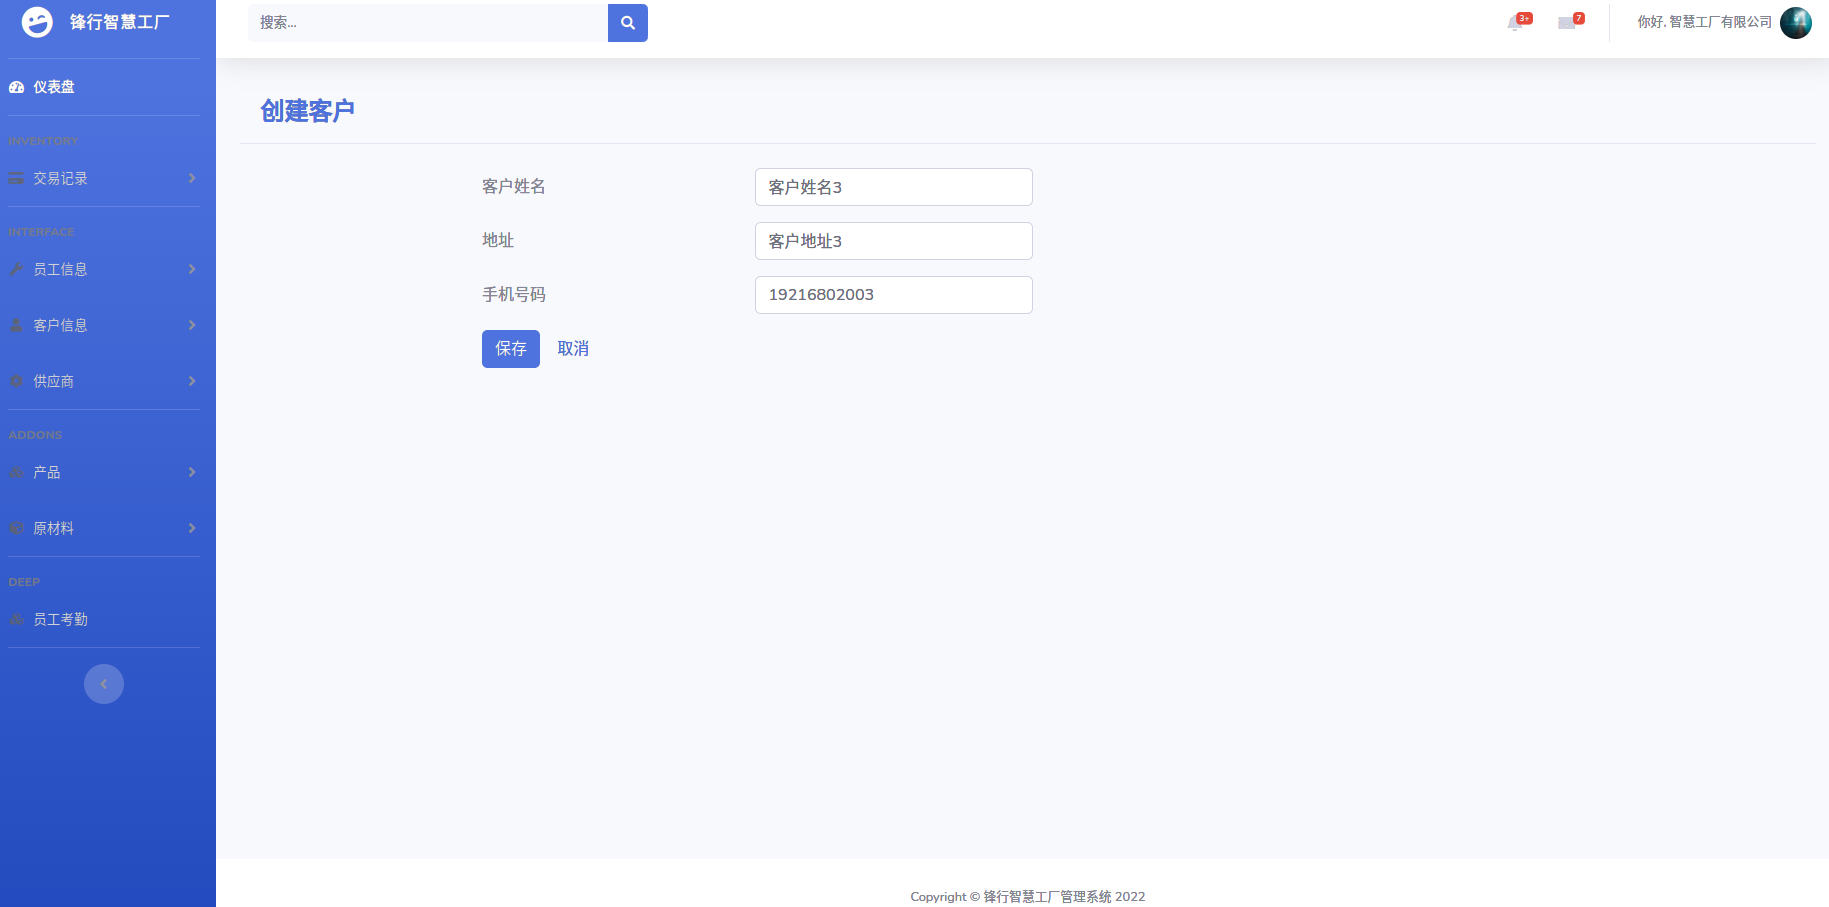
\includegraphics[width=\textwidth]{figures/6addnewcustomer.png}
        \subcaption{添加客户测试图}
        \label{fig:adnucstm}
    \end{subfigure}
    \\
    \begin{subfigure}{.35\textwidth}
        \centering
        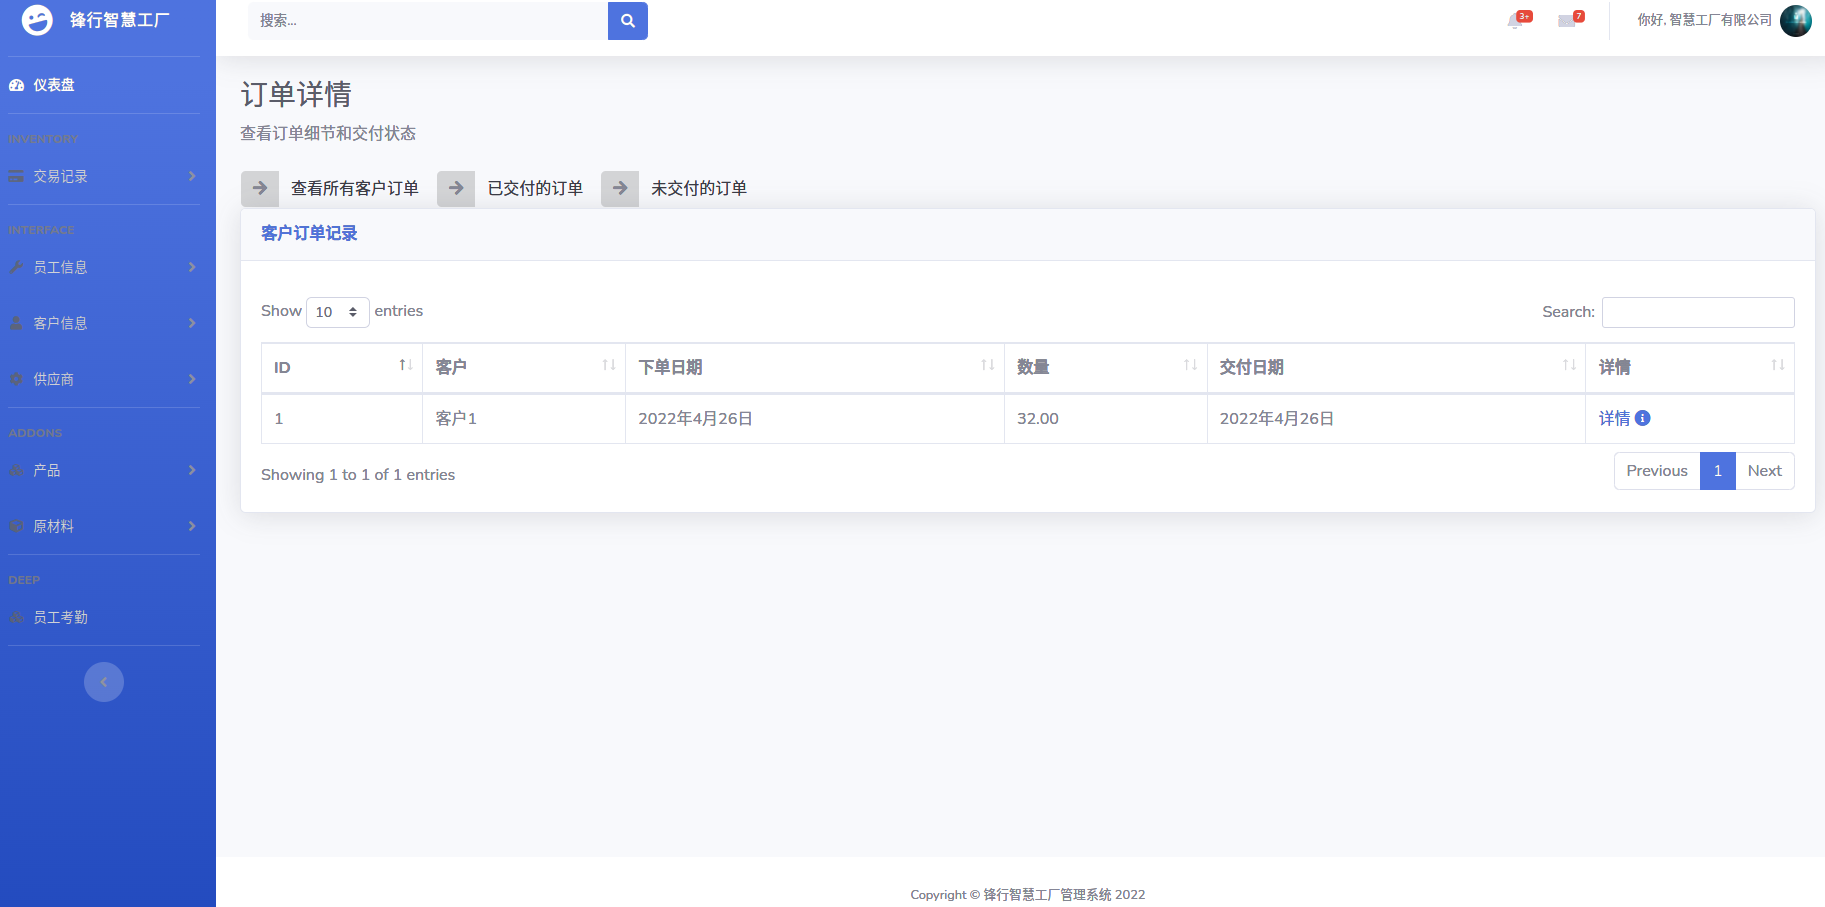
\includegraphics[width=\textwidth]{figures/6viewallorders.png}
        \subcaption{查看所有客户订单测试图}
        \label{fig:vuaods}
    \end{subfigure}
    \qquad
    \begin{subfigure}{.35\textwidth}
        \centering
        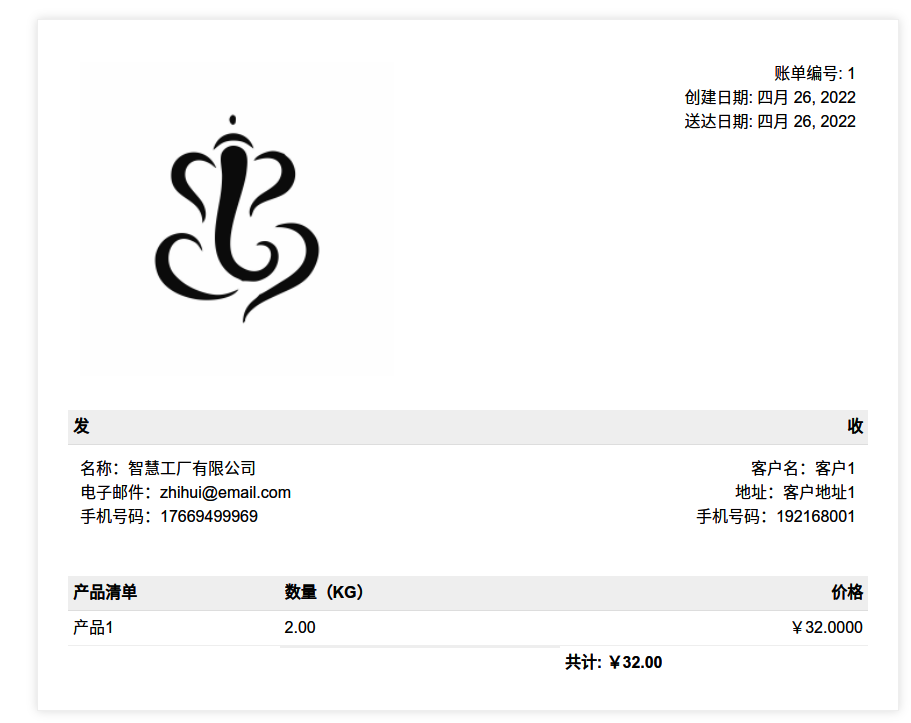
\includegraphics[width=\textwidth]{figures/6orderdetails.png}
        \subcaption{查看订单收据测试图}
        \label{fig:vuoddtls}
    \end{subfigure}
    \caption{客户信息管理测试图}
    \label{fig:cstmtst}
\end{figure}

同理,可对供应商信息、产品信息以及原材料信息进行查看与添加功能测试,如图\ref{fig:otstst}所示。图\ref{fig:vuaspie}为查看所有供应商信息,图\ref{fig:adspie}为添加供应商功能测试,图\ref{fig:vuaprdct}为查看所有产品信息详情,图\ref{fig:adnuprdct}为添加一类产品类型功能测试,图\ref{fig:vuamtra}为查看当前部门所有原材料信息详情,图\ref{fig:adnumtra}为添加原材料种类。

\begin{figure}[H]
    \centering
    \begin{subfigure}{.35\textwidth}
        \centering
        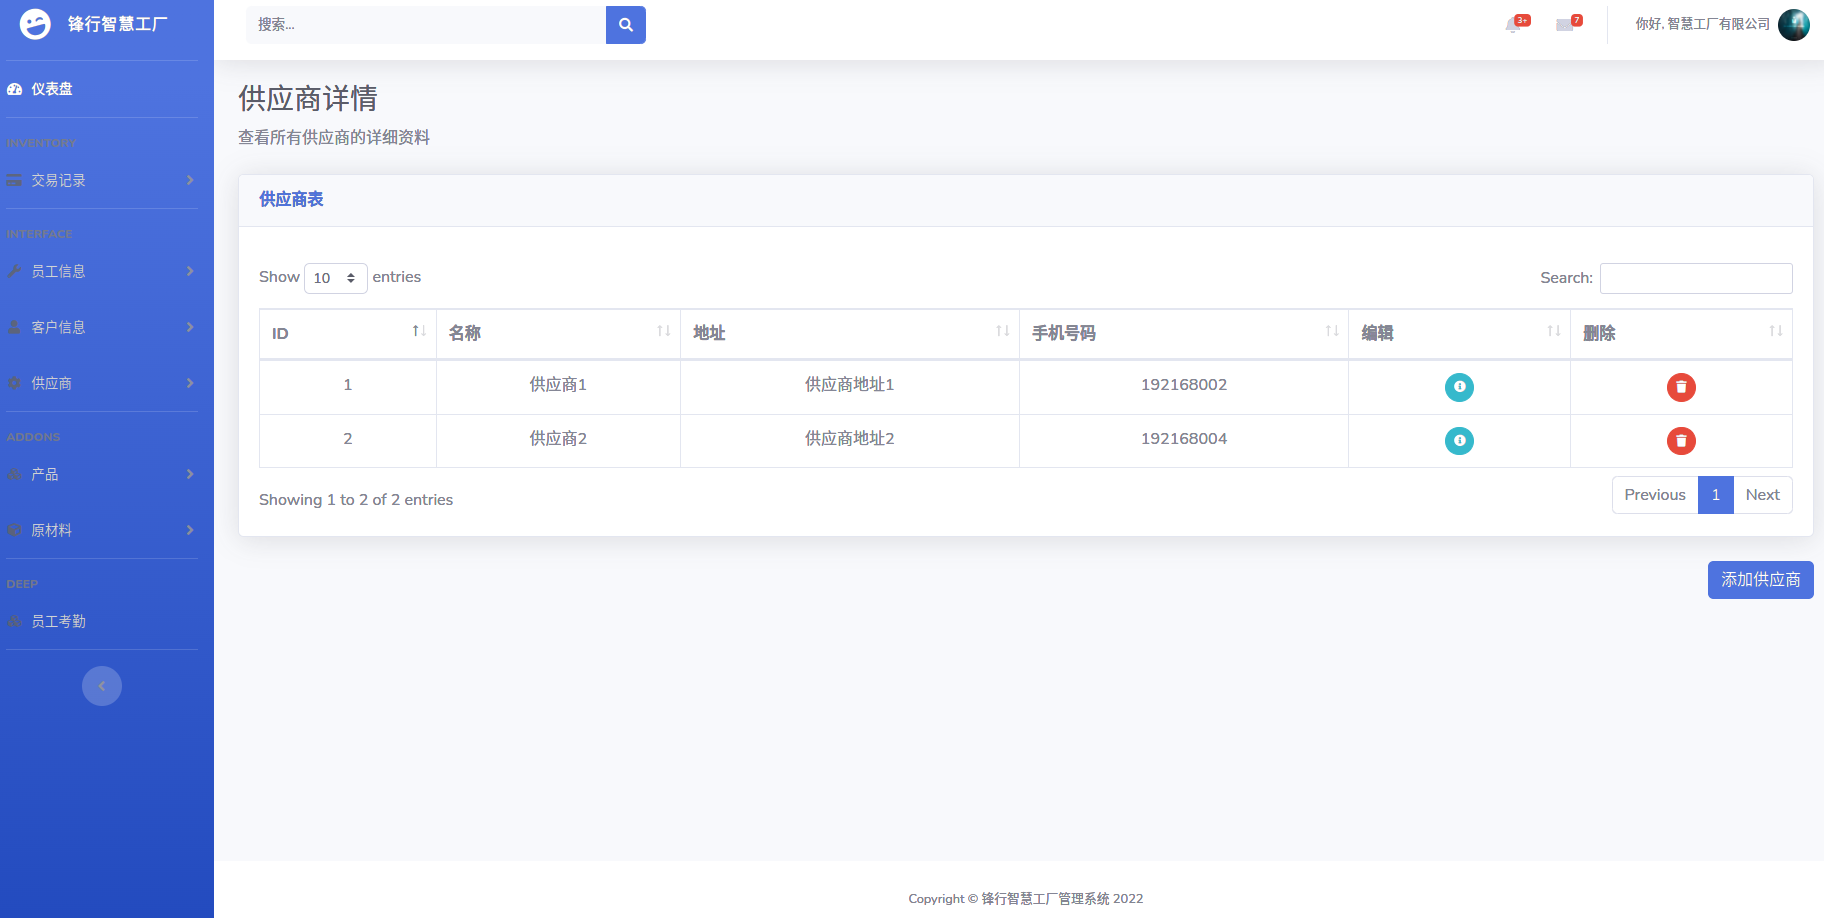
\includegraphics[width=\textwidth]{figures/6viewallsupplier.png}
        \subcaption{查看供应商信息详情图}
        \label{fig:vuaspie}
    \end{subfigure}
    \qquad
    \begin{subfigure}{.35\textwidth}
        \centering
        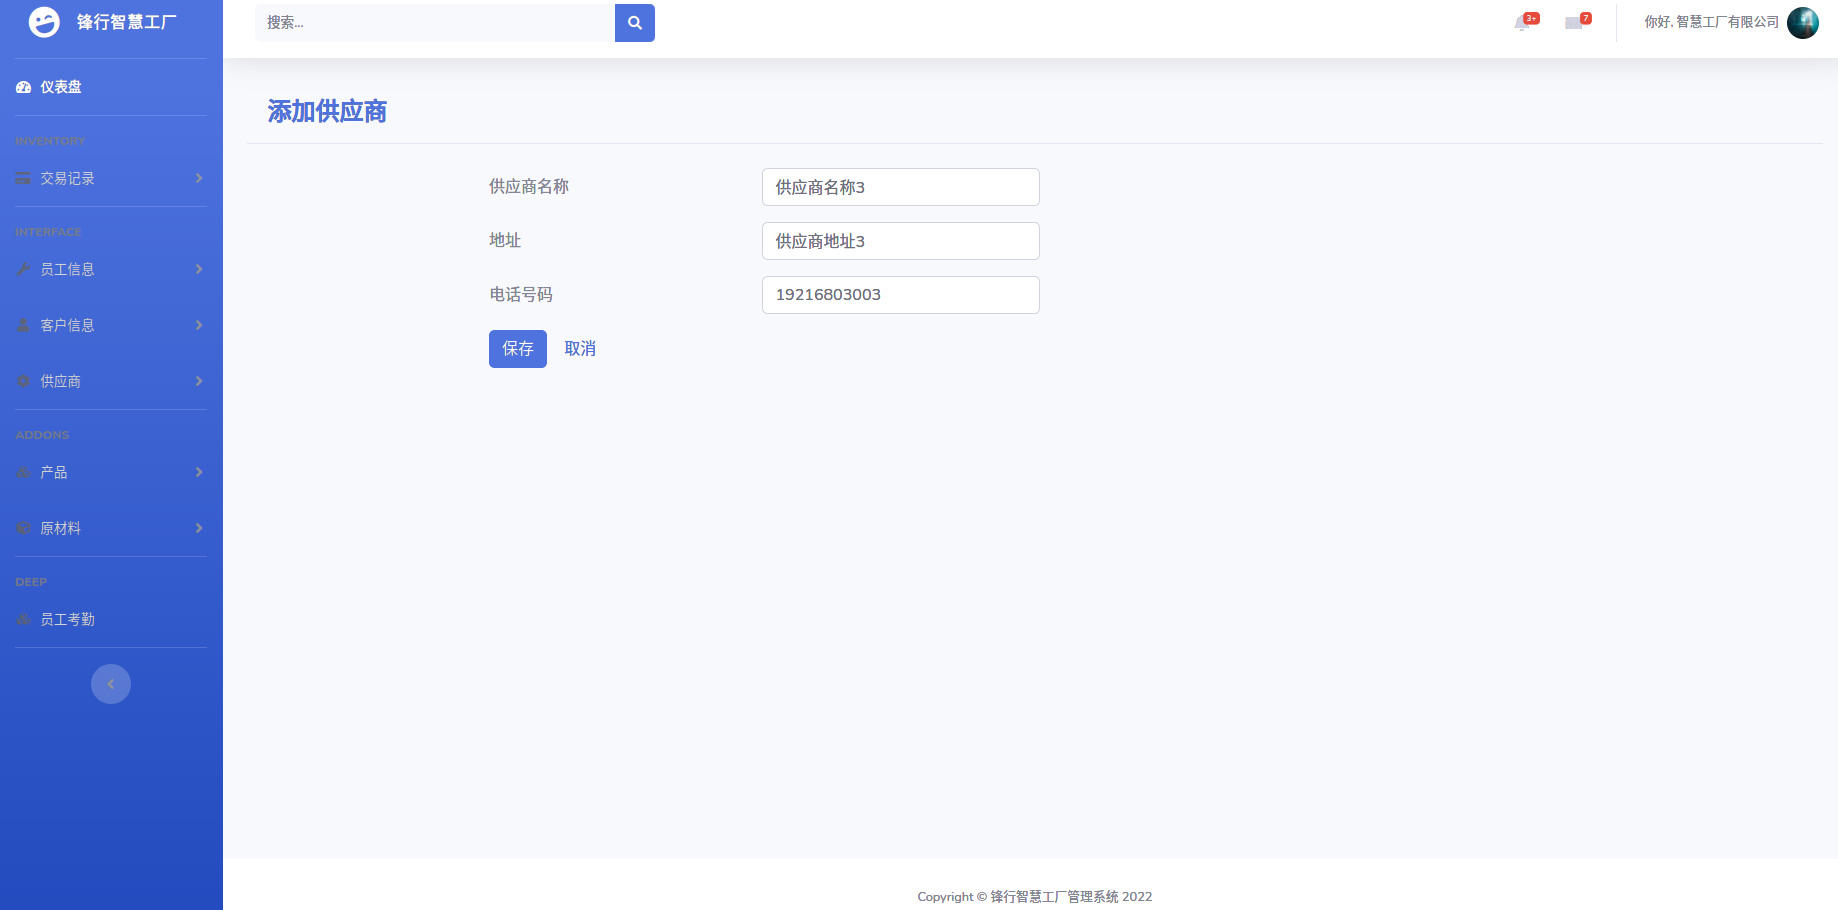
\includegraphics[width=\textwidth]{figures/6addnewsupplier.png}
        \subcaption{添加供应商测试图}
        \label{fig:adspie}
    \end{subfigure}
    \\
    \begin{subfigure}{.35\textwidth}
        \centering
        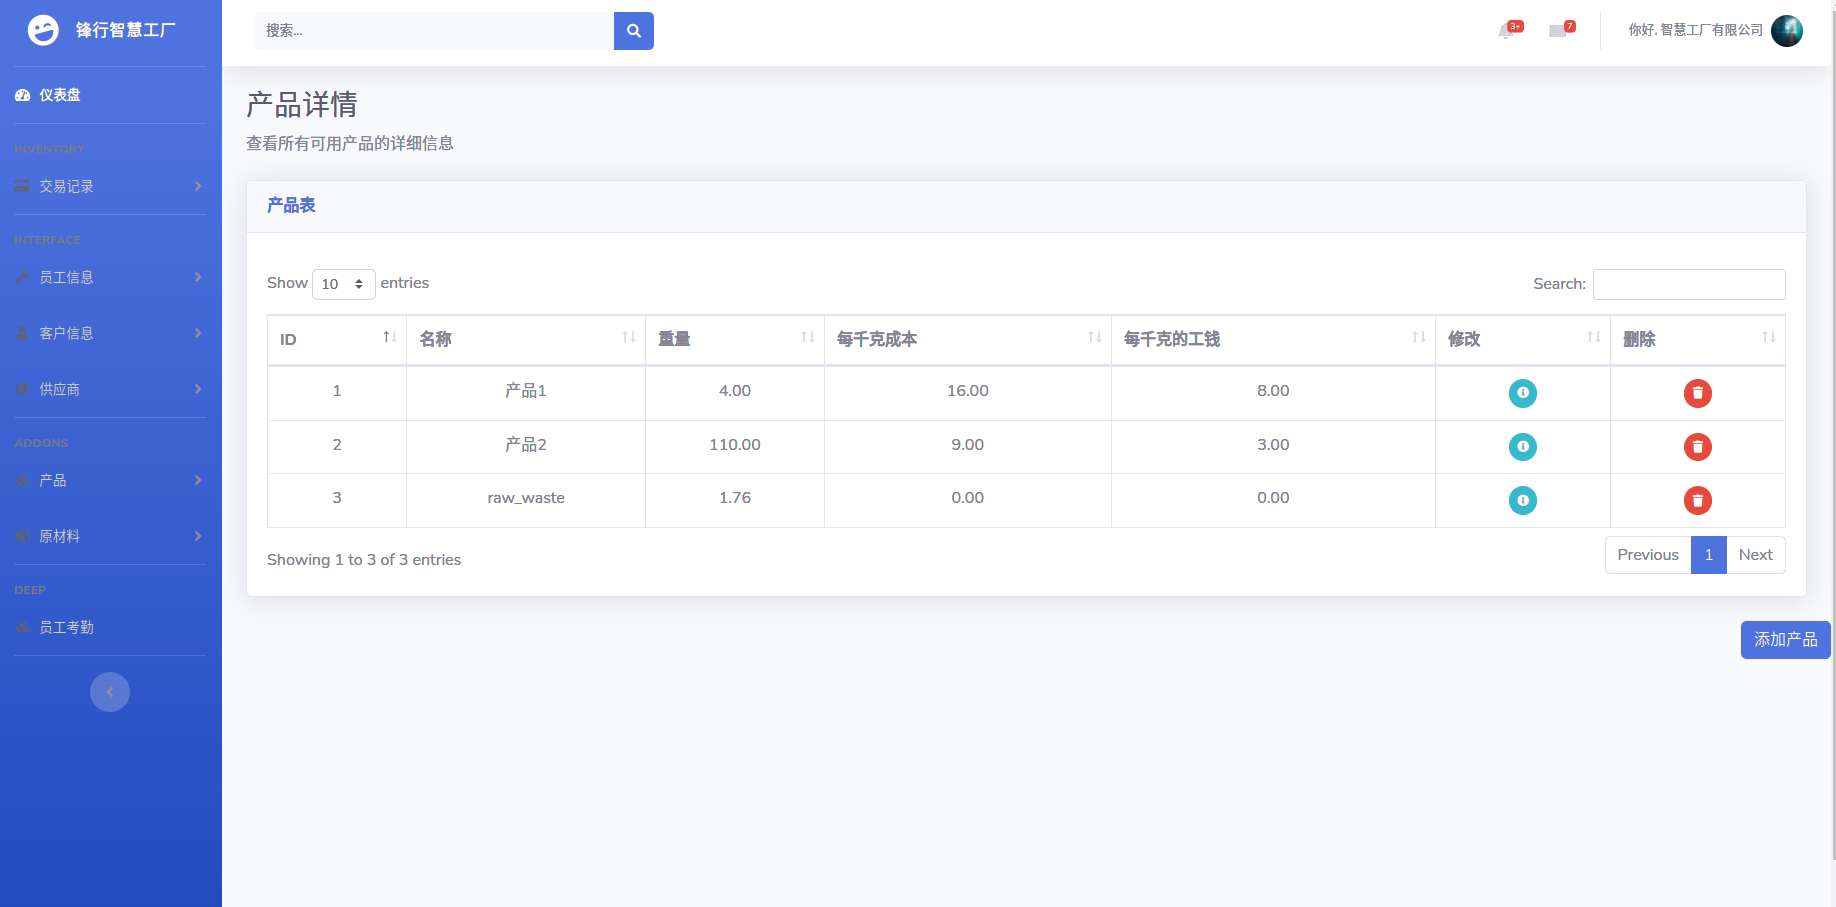
\includegraphics[width=\textwidth]{figures/6viewallproduct.png}
        \subcaption{查看所有产品详情测试图}
        \label{fig:vuaprdct}
    \end{subfigure}
    \qquad
    \begin{subfigure}{.35\textwidth}
        \centering
        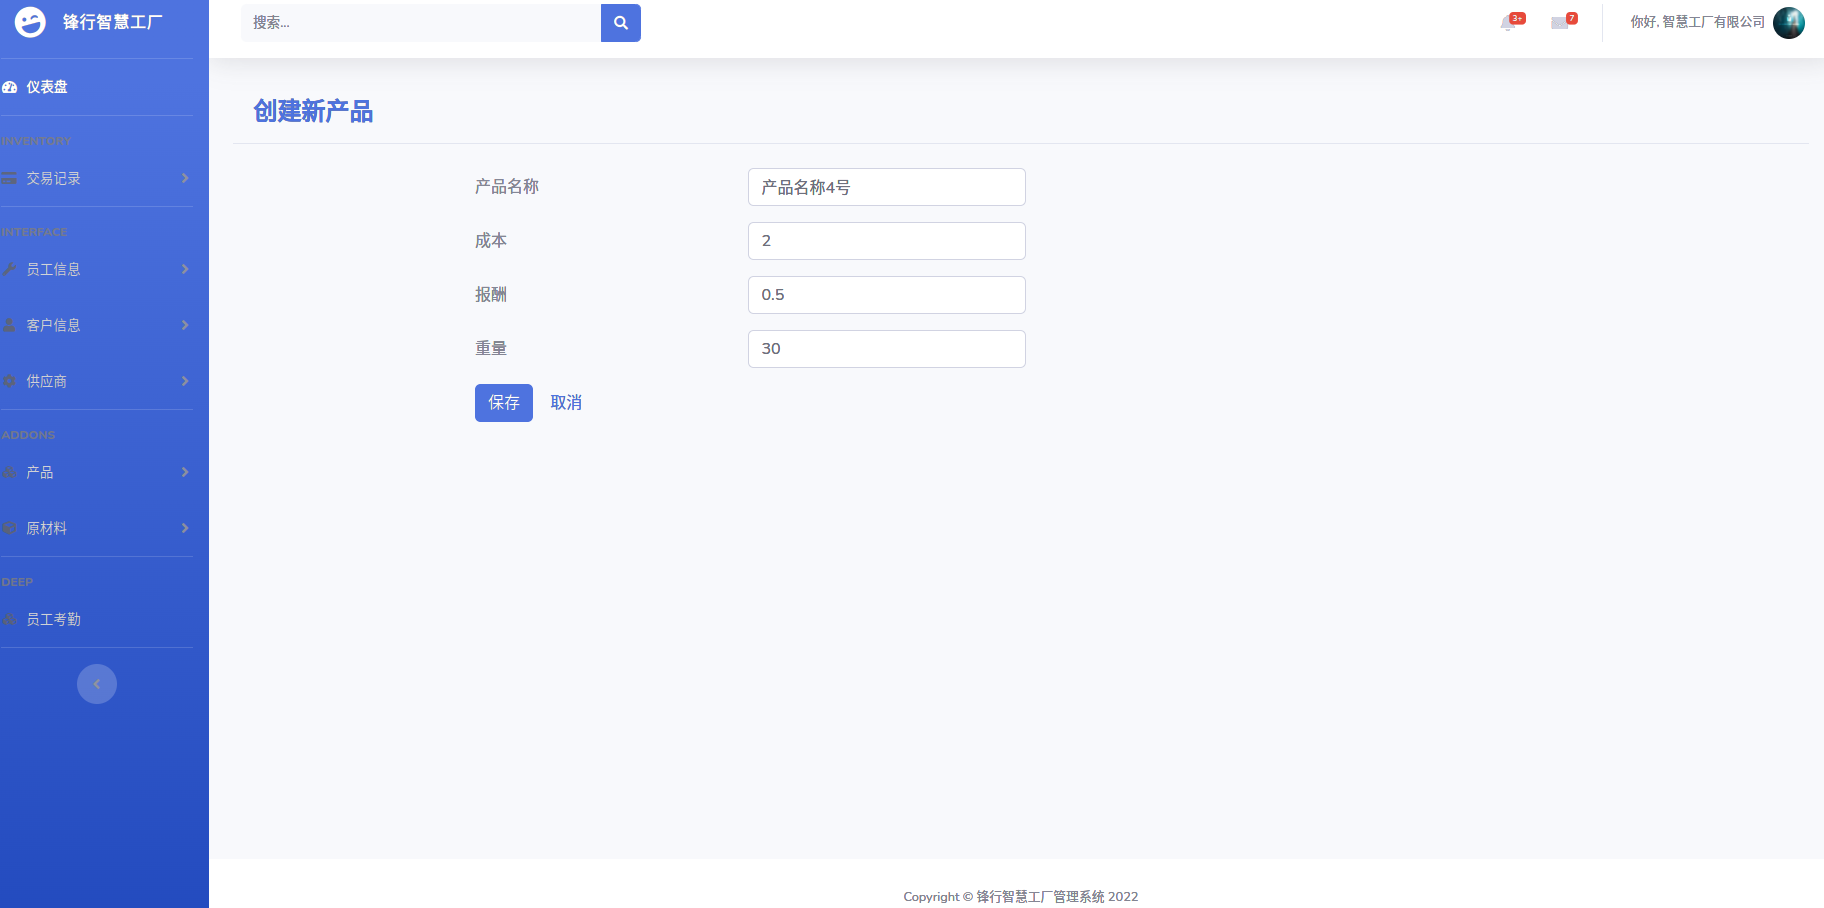
\includegraphics[width=\textwidth]{figures/6addnewproduct.png}
        \subcaption{添加新产品功能测试图}
        \label{fig:adnuprdct}
    \end{subfigure}
    \\
    \begin{subfigure}{.35\textwidth}
        \centering
        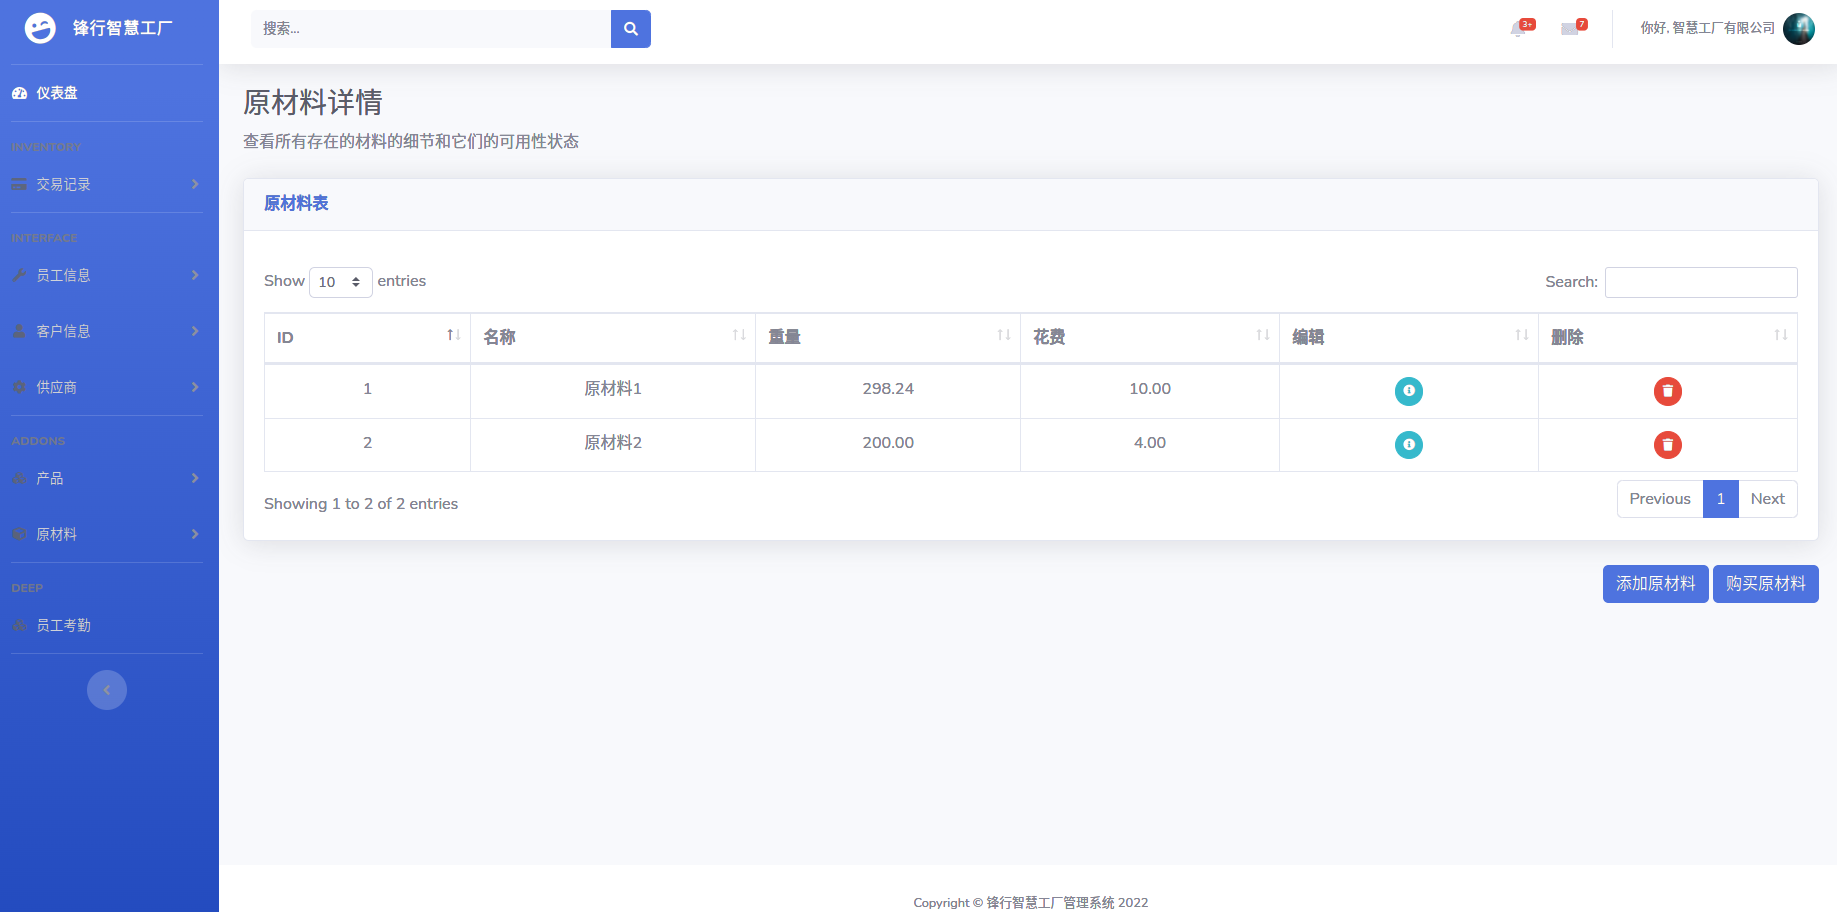
\includegraphics[width=\textwidth]{figures/6viewallmaterial.png}
        \subcaption{查看所有原材料详情测试图}
        \label{fig:vuamtra}
    \end{subfigure}
    \qquad
    \begin{subfigure}{.35\textwidth}
        \centering
        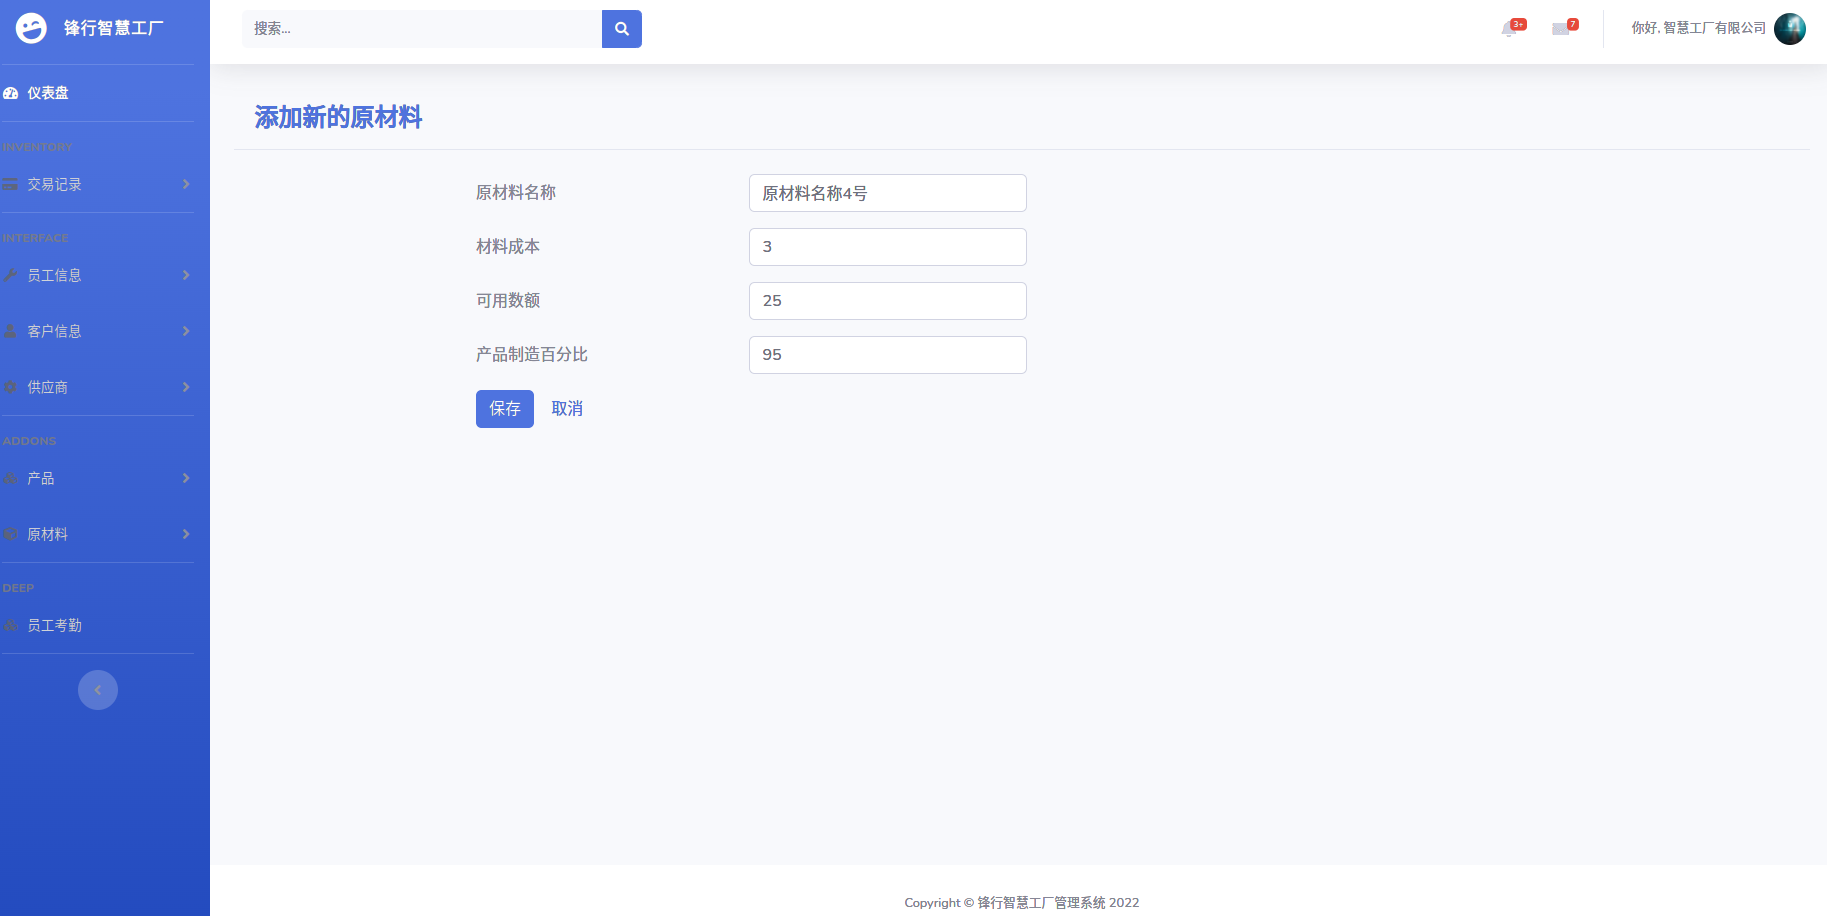
\includegraphics[width=\textwidth]{figures/6addnewmaterial.png}
        \subcaption{添加新原材料类型测试图}
        \label{fig:adnumtra}
    \end{subfigure}
    \caption{其它功能测试图}
    \label{fig:otstst}
\end{figure}

\subsection{员工考勤功能测试}

管理员进入员工考勤页面,首先查询当前的签到表记录并且将签到记录表展示在后台页面上,如图\ref{fig:empleatdc}所示。

\begin{figure}[H]
    \centering
    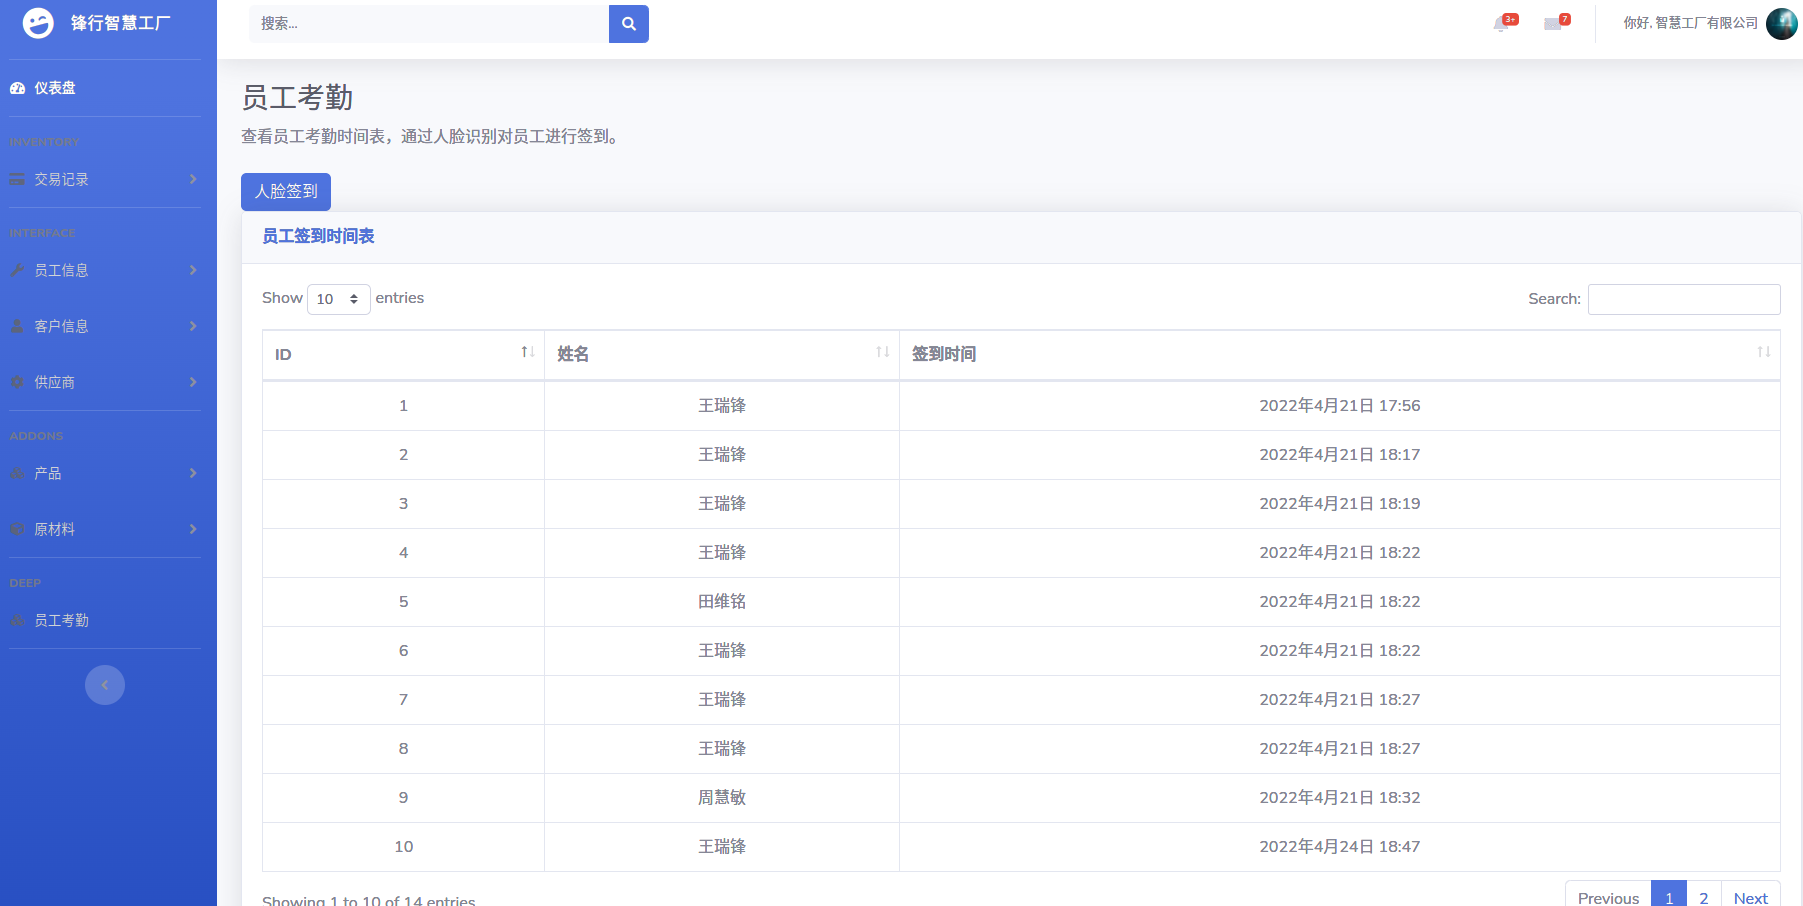
\includegraphics[width=.75\textwidth]{figures/6employeeattendance.png}
    \caption{员工考勤签到记录页面图}
    \label{fig:empleatdc}
\end{figure}

当点击人脸签到按钮时,首先调用摄像头对当前场景进行拍摄,并且将图像输入至人脸识别模块对人脸进行检测识别,如果在第一帧的时刻就已经识别出哪位员工在进行人脸签到,就直接向签到记录表中插入一条新签到记录,若人脸识别模块没有认出员工人脸图像,便打开一个摄像头窗口以便于人脸图像位置、姿势以及光照等调节,如图\ref{fig:fcrcgnttst}所示。图\ref{fig:fcrcgnt}为第一帧未能识别人脸图像之后弹出的摄像窗口以便于调整姿势、角度和光照等环境调节,图\ref{fig:mskdfcrcgnt}为佩戴口罩之后进行人脸识别签到测试。经过反复测试,该系统有着较高的准确率与较快的识别速度,可以应对日常工厂管理员工考勤场景。

\begin{figure}[H]
    \centering
    \begin{subfigure}{.45\textwidth}
        \centering
        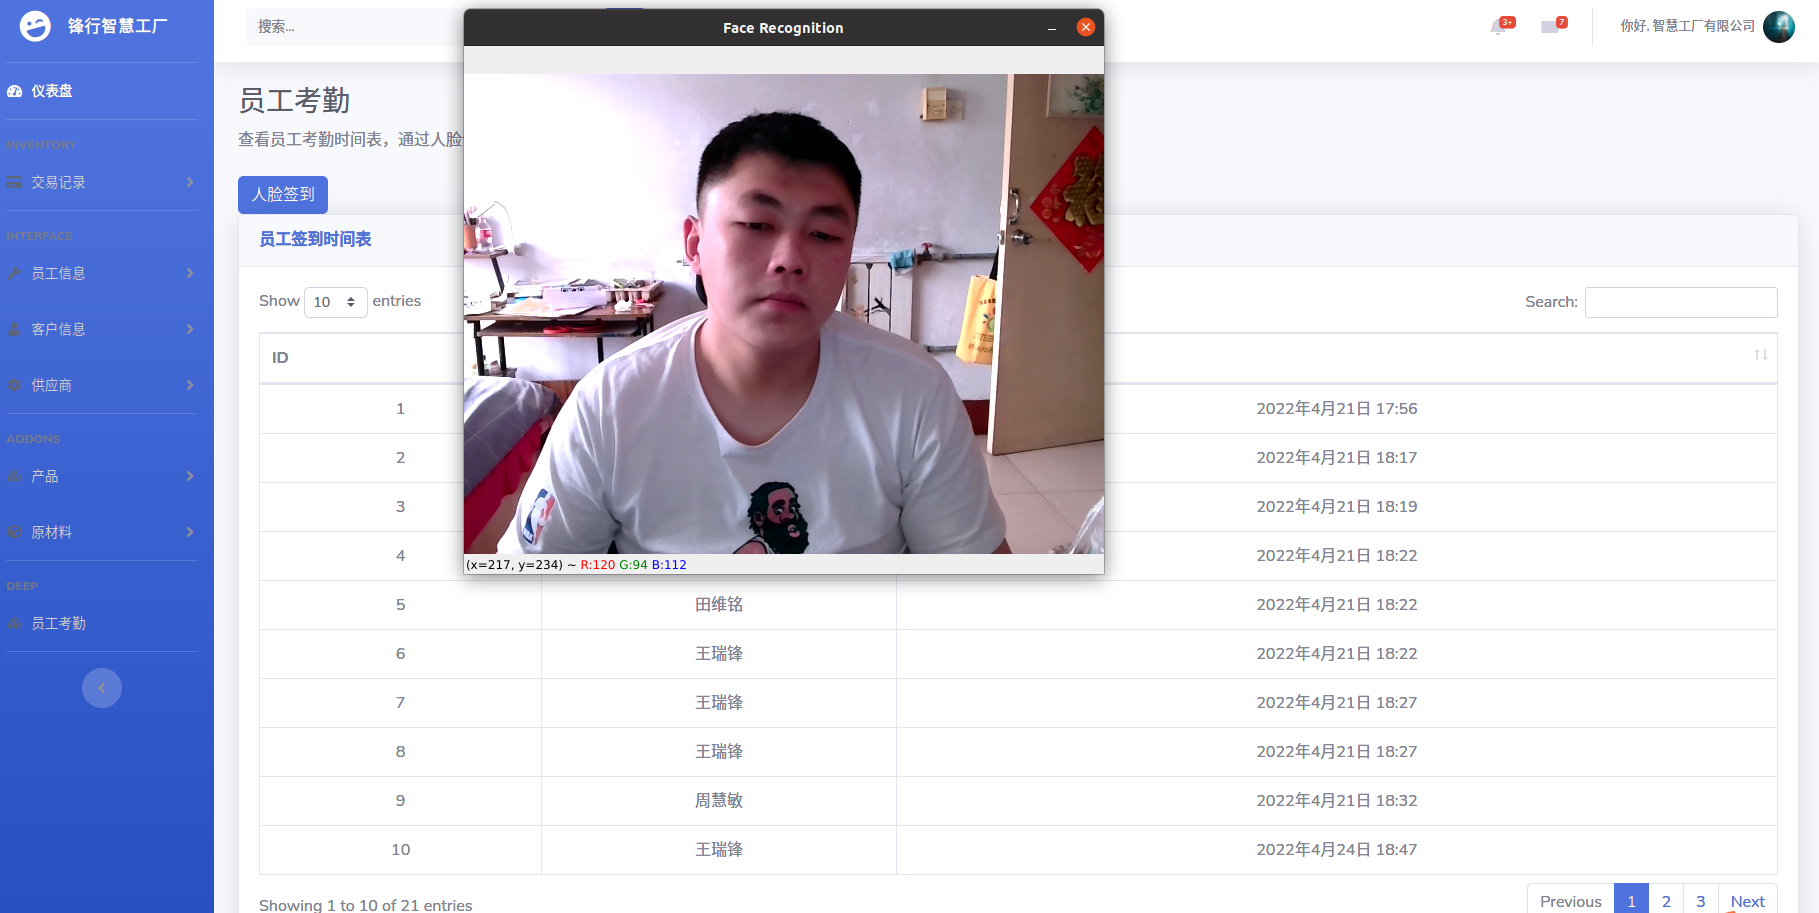
\includegraphics[width=\textwidth]{figures/6facerecerror.png}
        \subcaption{弹出摄像图像窗口图}
        \label{fig:fcrcgnt}
    \end{subfigure}
    \qquad
    \begin{subfigure}{.45\textwidth}
        \centering
        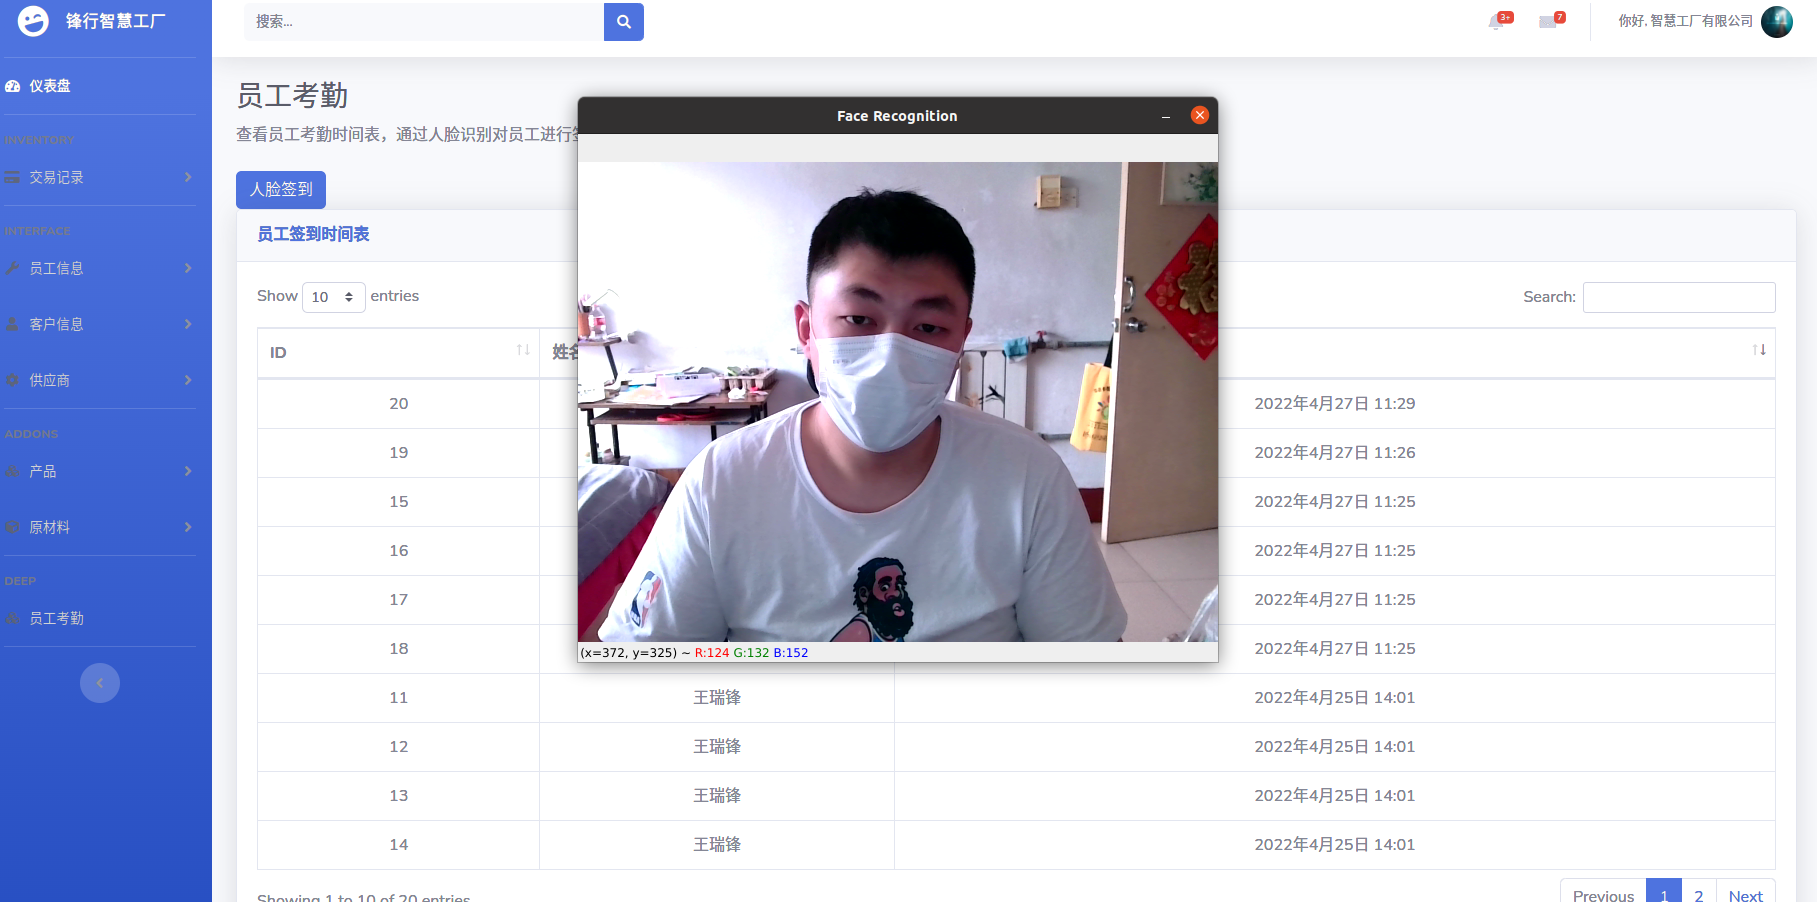
\includegraphics[width=\textwidth]{figures/6maskedfacerec.png}
        \subcaption{佩戴口罩人脸识别测试图}
        \label{fig:mskdfcrcgnt}
    \end{subfigure}
    \caption{人脸识别签到功能测试图}
    \label{fig:fcrcgnttst}
\end{figure}